\documentclass[11pt,aspectratio=169]{beamer}
\usetheme{Berlin}
\usepackage[utf8]{inputenc}
\usepackage[english]{babel}
\usepackage{amsmath}
\usepackage{amsfonts}
\usepackage{amssymb}
\usepackage{graphicx}
\usepackage{xcolor}
\usepackage{booktabs}
\usepackage{pgfpages}
\usepackage{tikz}
\usetikzlibrary{shapes,arrows,positioning,calc}
\author{Adam Aili \& Erik Ekelund}
\title{Model-Based Development of an Underwater Vehicle}
%\setbeamercovered{transparent} 
\setbeamertemplate{navigation symbols}{} 
%\logo{} 
%\institute{} 
\date{June 10} 
%\subject{} 
\setbeamertemplate{caption}{\insertcaption}
%\setbeameroption{show notes}
\setbeameroption{show notes on second screen=right}
\newcommand\scalemath[2]{\scalebox{#1}{\mbox{\ensuremath{\displaystyle #2}}}}
\begin{notation}% Passing the option "old" to the notation environment will redefine the notationtabular environment so that it produces an old style LaTeX tabular instead of a ctable.sty style tabular.
  \centering
  
% Lägg in förkortningarna i bokstavsordning!
  \begin{notationtabular}{Abbreviations}{Abbreviation}{Description}
    \abbrCB\index{CB@\abbrCG!abbreviation} & Center of buoyancy. \\
    \abbrCG\index{CG@\abbrCG!abbreviation} & Center of gravity. \\
    \abbrCO\index{CO@\abbrCO!abbreviation} & Center of origin. \\
    \abbrDOF\index{DOF@\abbrDOF!abbreviation} & Degrees of freedom. \\
    \abbrEKF\index{EKF@\abbrEKF!abbreviation} & Extended Kalman filter.\\
    \abbrESC\index{ESC@\abbrESC!abbreviation} & Electronic speed controller.\\
    \abbrIMU\index{IMU@\abbrIMU!abbreviation} & Inertial measurement unit.\\
    \abbrIO\index{I/O@\abbrIO!abbreviation}   & Input/Output.\\
    \abbrKF\index{KF@\abbrKF!abbreviation}	& Kalman filter.\\
    \abbrMPC\index{MPC@\abbrMPC!abbreviation} & Model predictive control.\\
    \abbrPID\index{PID@\abbrPID!abbreviation} & Proportional, integral, differential (regulator). \\
    \abbrPI\index{PI@\abbrPI!abbreviation} & Proportional, integral (regulator). \\
    \abbrRPM\index{RPM@\abbrRPM!abbreviation} & Rotations per minute. \\
    \abbrSLAM\index{SLAM@\abbrSLAM!abbreviation} & Simultaneous localisation and mapping. \\
    \abbrSNR\index{SNR@\abbrSNR!abbreviation} & Signal to noise ratio. \\
    \abbrROS\index{ROS@\abbrROS!abbreviation} & Robot Operating System. \\
    \abbrROV\index{ROV@\abbrROV!abbreviation} & Remotely operated vehicle. \\
    \abbrUV\index{UV@\abbrUV!abbreviation} & Unmanned vehicle. \\

    
    
  \end{notationtabular}
  
\end{notation}


\begin{document}


\begin{frame}
\titlepage
\end{frame}
%%%%%%%%%%%%%%%%%%%%%Intro%%%%%%%%%%%%%%%%%%%%%%%%%%%%%%%%%%%%%%%%%%%%%%%%%%%%%%%%%%%%%%%%%%%%%%%%%
\begin{frame}
\begin{itemize}
\item Model-based design development
\item Control system
\end{itemize}
\note{\begin{itemize}
\item Purpose of model-based design development
\item Purpose of a control system
\end{itemize}}
\end{frame}

\begin{frame}
\begin{itemize}
\item Assemble the ROV
\item Develop a framework for changing controller in the ROV
\item Estimate a model of the ROV
\item Create a plant model of the ROV in Matlab/Simulink
\item Develop a robust model-based controller and evaluate its performance with simulations and tests
\end{itemize}
\note{Goals for the thesis}
\end{frame}


%%%%%%%%%%%%%%%%%%%%%Rov platfrom%%%%%%%%%%%%%%%%%%%%%%%%%%%%%%%%%%%%%%%%%%%%%%%%%%%%%%%%%%%%%%%%%%
\section{ROV Platform}
\begin{frame}
\begin{columns}
\begin{column}{0.5\textwidth}
\begin{itemize}
\item BlueROV package from Blue Robotics
\item Raspberry Pi 2
\item Raspicam
\item HkPilot 2.7
\end{itemize}
\end{column}
\begin{column}{0.5\textwidth}
\begin{figure}
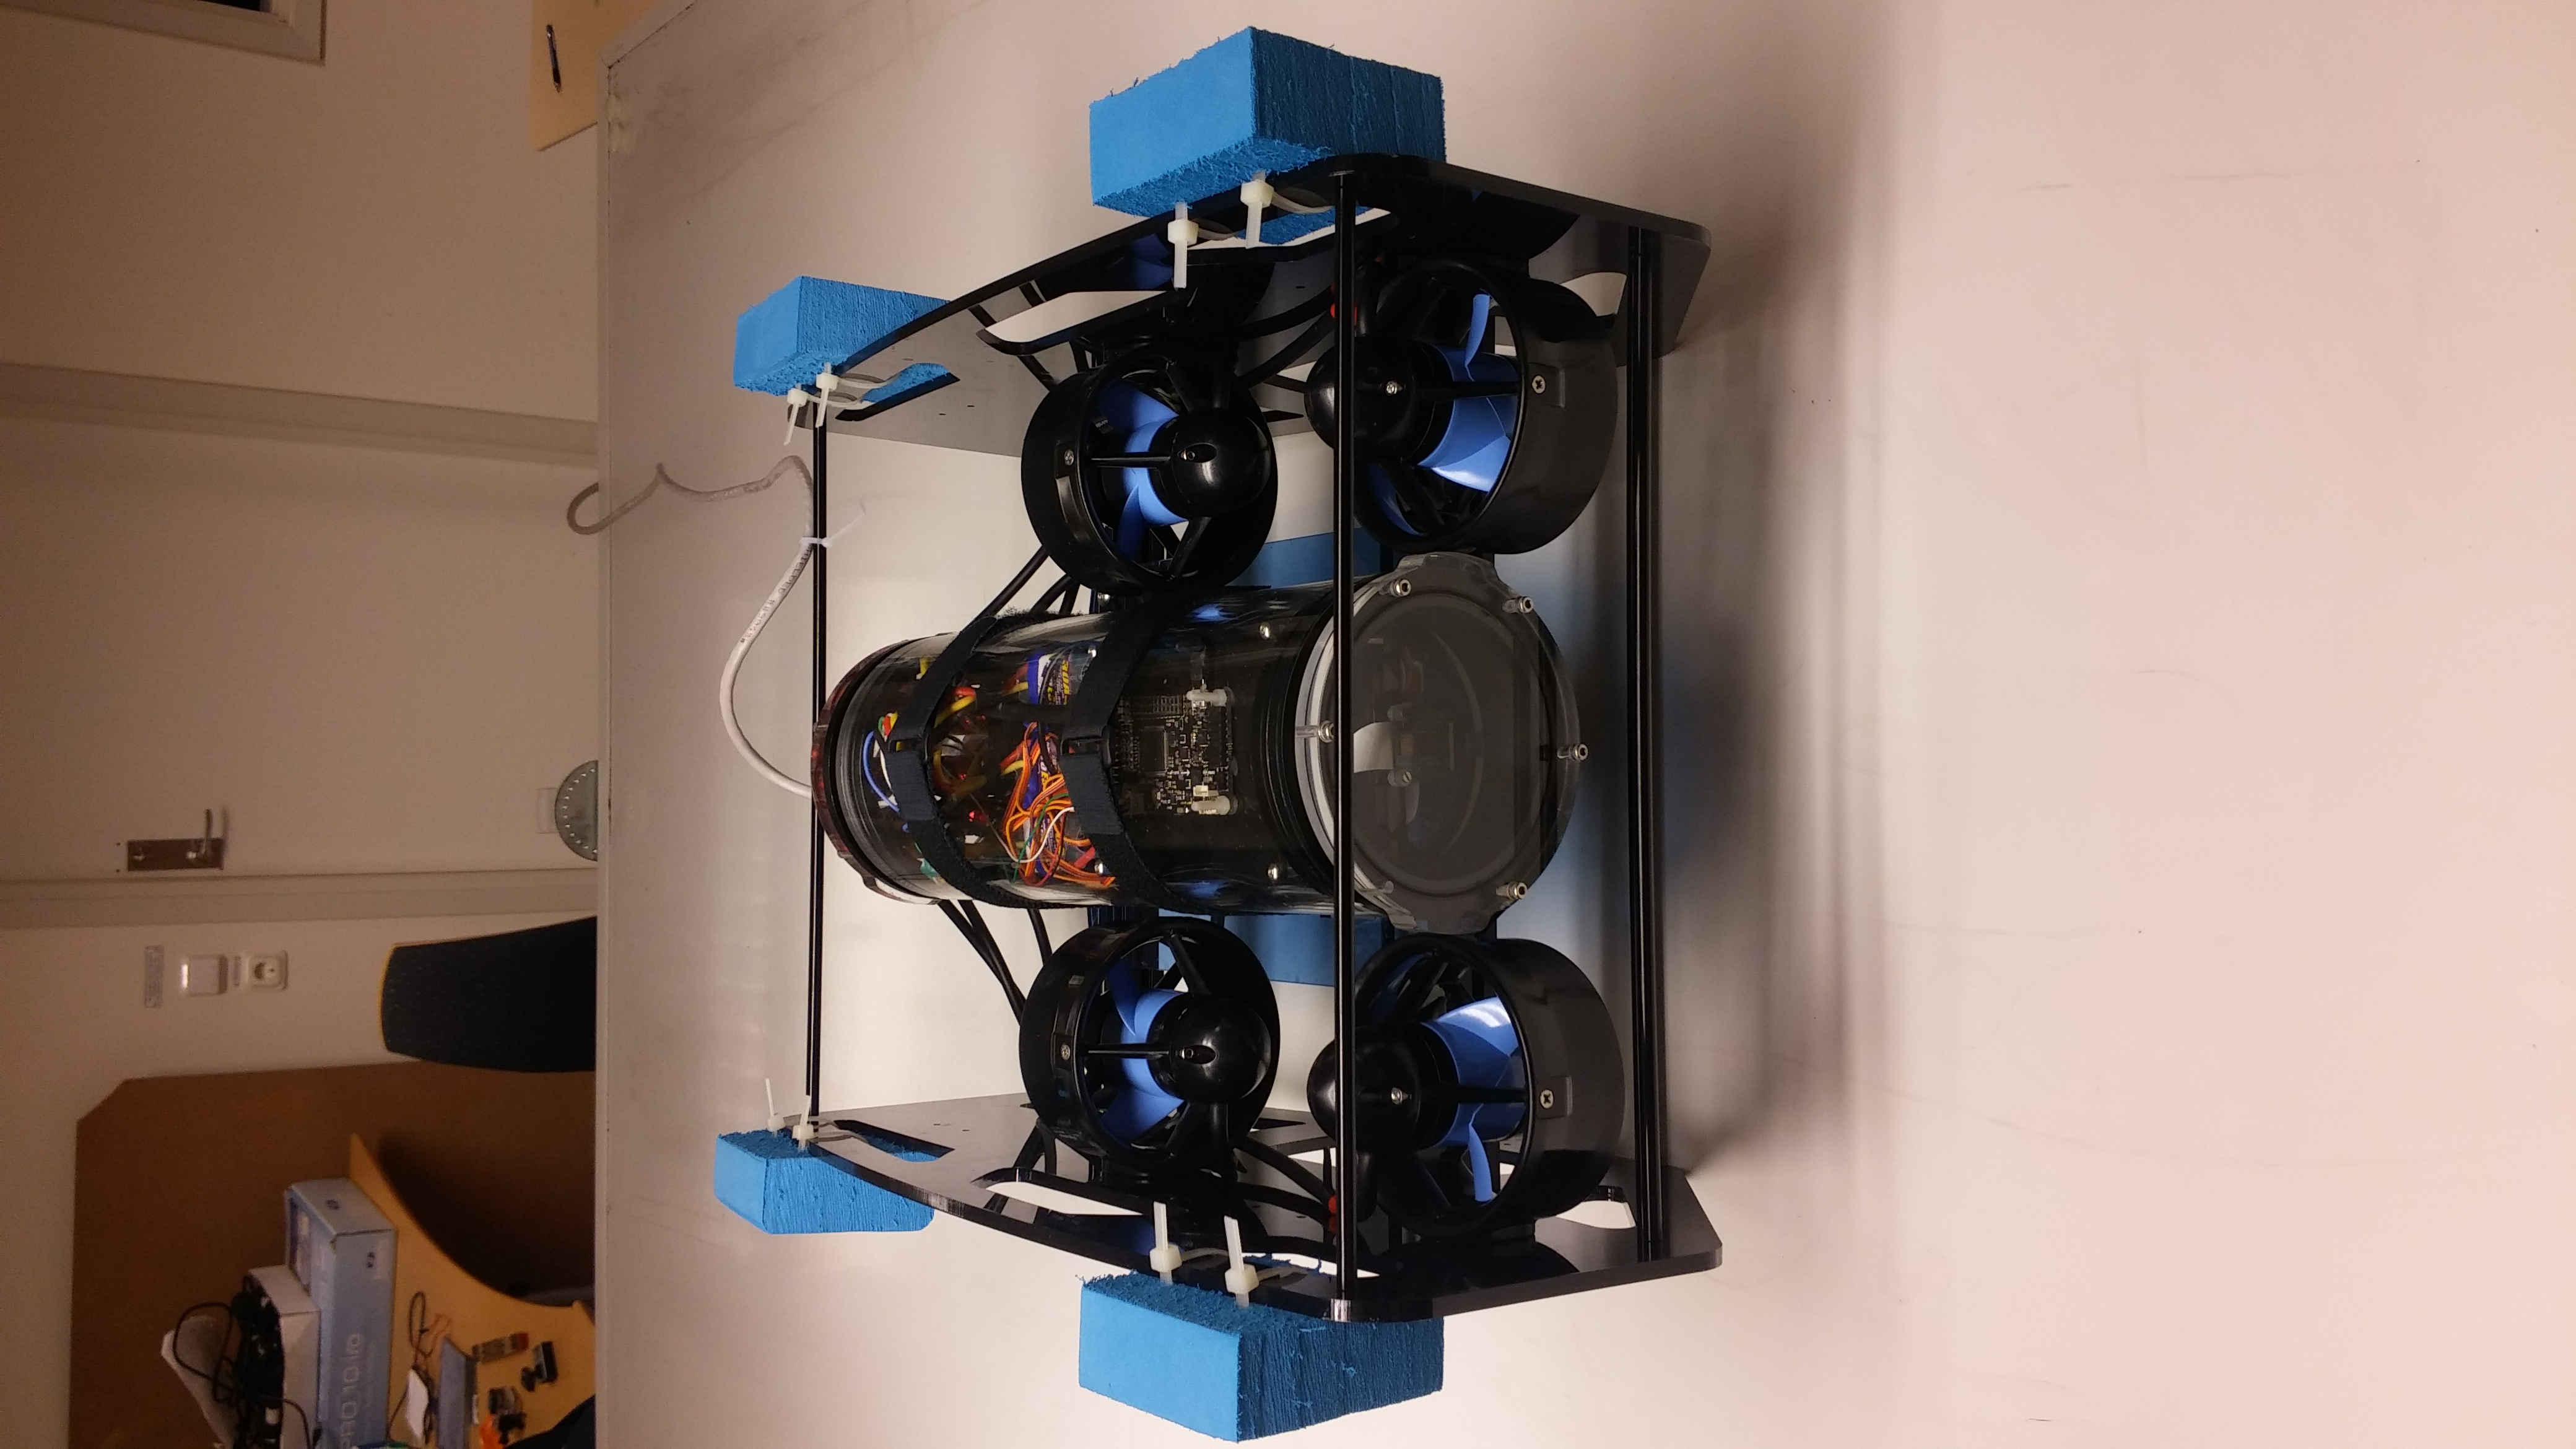
\includegraphics[trim={40cm 0cm 45cm 0cm},clip,angle=270,width=\textwidth]{fig/bluerov}
\end{figure}
\end{column}
\end{columns}

\note{\begin{itemize}
\item The blueROV package from Blue Robotics comes with 6 thrusters, 6 ESC:s and an acrylic tube.
\item The on-board computer is the Raspberry Pi 2 which communicates with the workstation and perform controller calculations.
\item The camera is used to get live video.
\item HkPilot 2.7 is based on a multicopter autopilot. The HkPilot has three on-chip sensors: barometer, IMU and magnetometer. An external pressure sensor is wired to the HkPilot via I2C
\end{itemize}
}
\end{frame}

\begin{frame}
\begin{figure}
	\centering
		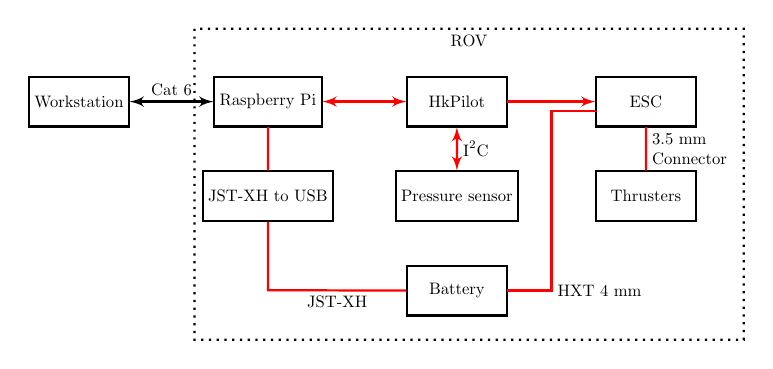
\begin{tikzpicture}[auto, thick, node distance=2cm,>=latex',
			 block/.style  = {draw, rectangle,minimum height=3em, minimum width=6em},
			 sum/.style    = {draw, circle, inner sep=0pt, text width=4mm,align=center, node distance=1cm},
			 input/.style  = {coordinate},
			 output/.style = {coordinate},
			 pinstyle/.style = {pin edge={to-,thin,black}}, scale=0.6, every node/.style={transform shape}]
			 
			 \node [block, node distance=5cm] (ws) {Workstation};
			 \node [block, right of=ws, node distance=4cm] (rasp) {Raspberry Pi};
			 \node [block, right of=rasp, node distance=4cm] (HkPilot) {HkPilot};
			 \node [block, right of=HkPilot, node distance=4cm] (esc) {ESC};
			 \node [block, below of=esc, node distance=2cm] (thrust) {Thrusters};
			 \node [block, below of=HkPilot] (pressure) {Pressure sensor};
			 \node [block, below of=rasp] (diag) {JST-XH to USB};
			 \node [block, below of=pressure] (bat) {Battery};
			 
			 
			 \draw[<->, thick] (ws) -- node[above]{Cat 6} (rasp);
			 \draw[thick,red] (rasp) -- node[right]{\color{black} \abbrUSB} (diag);
			 \draw[thick,red] (diag.south) -- ++(0,-1.45)-- node[below]{\color{black} JST-XH} (bat.west);
			 \draw[<->, thick,red] (rasp) -- node[above]{\color{black} \abbrUSB} (HkPilot);
			 \draw[<->, thick,red] (HkPilot) -- node[right]{\color{black} $\text{I}^2\text{C}$} (pressure);
			 \draw[->, thick,red] (HkPilot) -- node[above]{\color{black} \abbrPWM} (esc);
			 \draw[thick,red] (esc) -- node[right,align=left]{\color{black} 3.5 mm \\ \color{black} Connector} (thrust);
			 \draw[thick,red] (bat) -| node[right]{\color{black} HXT 4 mm} ++(2,3.8) -|  ($ (esc.west)+(0,-0.2)$);
			 
			 \node[coordinate, above left = 1cm and 0.4cm of rasp](tl){};
			 \node[coordinate, below left = 4.5cm and 0.4cm of rasp](bl){};
			 \node[coordinate, below right = 2.5cm and 1cm of thrust](br){};
			 \node[coordinate, above right = 1cm and 1cm of esc](tr){};
			 
			 \draw[dotted] (tl) -- (bl) -- (br) -- (tr) -- node[below]{ROV} (tl);
		\end{tikzpicture}
\end{figure} 
\note{\begin{itemize}
\item The schematic of the ROV
\item Workstation runs sensor fusion, operator inputs and visualisation. 
\item The Raspberry Pi runs the controller node and inter communication with the other computers.
\item HkPilot samples sensors and sends thruster signals.
\end{itemize}}
\end{frame}
%%%%%%%%%%%%%%%%%%%%%Model%%%%%%%%%%%%%%%%%%%%%%%%%%%%%%%%%%%%%%%%%%%%%%%%%%%%%%%%%%%%%%%%%%
\section{Modelling the ROV}
\begin{frame}{Coordinate systems}
\begin{itemize}
\item What is a model and how can it be used?
\item Notation
\item Coordinate systems
\end{itemize}
\newcommand*{\coordinateRadius}{0.05}
\newcommand*{\coordRot}{30}
\begin{figure}
    \centering
    \begin{tikzpicture}[scale=2]
        \pgfmathsetmacro\by{\coordinateRadius*sin(45)}
        \pgfmathsetmacro\bx{\coordinateRadius*cos(45)}
        \pgfmathsetmacro\ay{\coordinateRadius*sin(\coordRot)}
        \pgfmathsetmacro\ax{\coordinateRadius*cos(\coordRot)}
        \pgfmathsetmacro\coordYRot{sin(\coordRot)}
        \pgfmathsetmacro\coordXRot{cos(\coordRot)}
        
        \coordinate (O) at (0,0);
        \draw[thick,->] (O) ++(\coordinateRadius,0) -- ++(1,0) node[anchor=north east]{$\north$};
        \draw[thick,->] (O) ++(0,-\coordinateRadius)-- ++(0,-1) node[anchor=south east]{$\east$};
        \draw (O) circle (0.05) node[anchor=south,]{$\down$,\color{blue}$z''$};
        \draw (O) -- ++(\bx,\by) (O) -- ++(-\bx,-\by) (O) -- ++(-\bx,\by) (O)  -- ++(\bx,-\by);
        
        \draw[thick,blue,->] (O) ++(\ax,-\ay) -- ++(\coordXRot,-\coordYRot) node[anchor=north west]{$x''$ };
        \draw[thick,blue,->] (O) ++(-\ay,-\ax) -- ++(-\coordYRot,-\coordXRot) node[anchor=north east]{$y''$};
        \draw[->] (O) ++(0.5,0) arc (0:-\coordRot:0.5) node[right]{\yawAngle};
        
        \def\coordDistance{1.5}
        
         \coordinate (O) at (\coordDistance,0);
         \draw[blue,thick,->] (O) ++(\coordinateRadius,0) -- ++(1,0) node[anchor=north east]{$x''$};
         \draw[blue,thick,->] (O) ++(0,-\coordinateRadius)-- ++(0,-1) node[anchor=south east]{$z''$};
         \draw (O) circle (0.05) node[anchor=south,]{{\color{blue}$y''$},\color{gray}$y'$};
         \draw[fill=black] (O) circle (0.0125);
        
         \draw[thick,gray,->] (O) ++(\ax,\ay) -- ++(\coordXRot,\coordYRot) node[anchor=south west]{$x'$};
         \draw[thick,gray,->] (O) ++(\ay,-\ax) -- ++(\coordYRot,-\coordXRot) node[anchor=north east]{$z'$};
         \draw[->] (O) ++(0.5,0) arc (0:\coordRot:0.5) node[right]{\pitchAngle};
         
          
        \pgfmathsetmacro\coordDistanceZ{2*\coordDistance+1}
        
         \coordinate (O) at (\coordDistanceZ,0);
         \draw[thick,gray,->] (O) ++(-\coordinateRadius,0) -- ++(-1,0) node[anchor=north west]{$y'$};
         \draw[thick,gray,->] (O) ++(0,-\coordinateRadius) -- ++(0,-1) node[anchor=south east]{$z'$};
         \draw (O) circle (0.05) node[anchor=south,]{{\color{gray}$x'$},\color{red}$x$};
         \draw[fill=black] (O) circle (0.0125);
        
        \draw[thick,red,->] (O) ++(\ay,-\ax) -- ++(\coordYRot,-\coordXRot) node[anchor=north west]{$z$};
        \draw[thick,red,->] (O) ++(-\ax,-\ay) -- ++(-\coordXRot,-\coordYRot) node[anchor=south east]{$y$};
        \draw[->] (O) ++(-0.5,0) arc (180:180+\coordRot:0.5) node[left]{\rollAngle};
    
    \end{tikzpicture}
\end{figure}

\note{\begin{itemize}
\item What is a model?
\item What is a model used for?
\end{itemize}}
\end{frame}

\begin{frame}
\begin{columns}
\newcommand*{\coordinateRadius}{0.05}
\newcommand*{\coordRot}{30}
\begin{column}{0.5\textwidth}
\begin{figure}
    \centering
 \begin{tikzpicture}
    \node[anchor=south west,inner sep=0] (image) at (0,0) {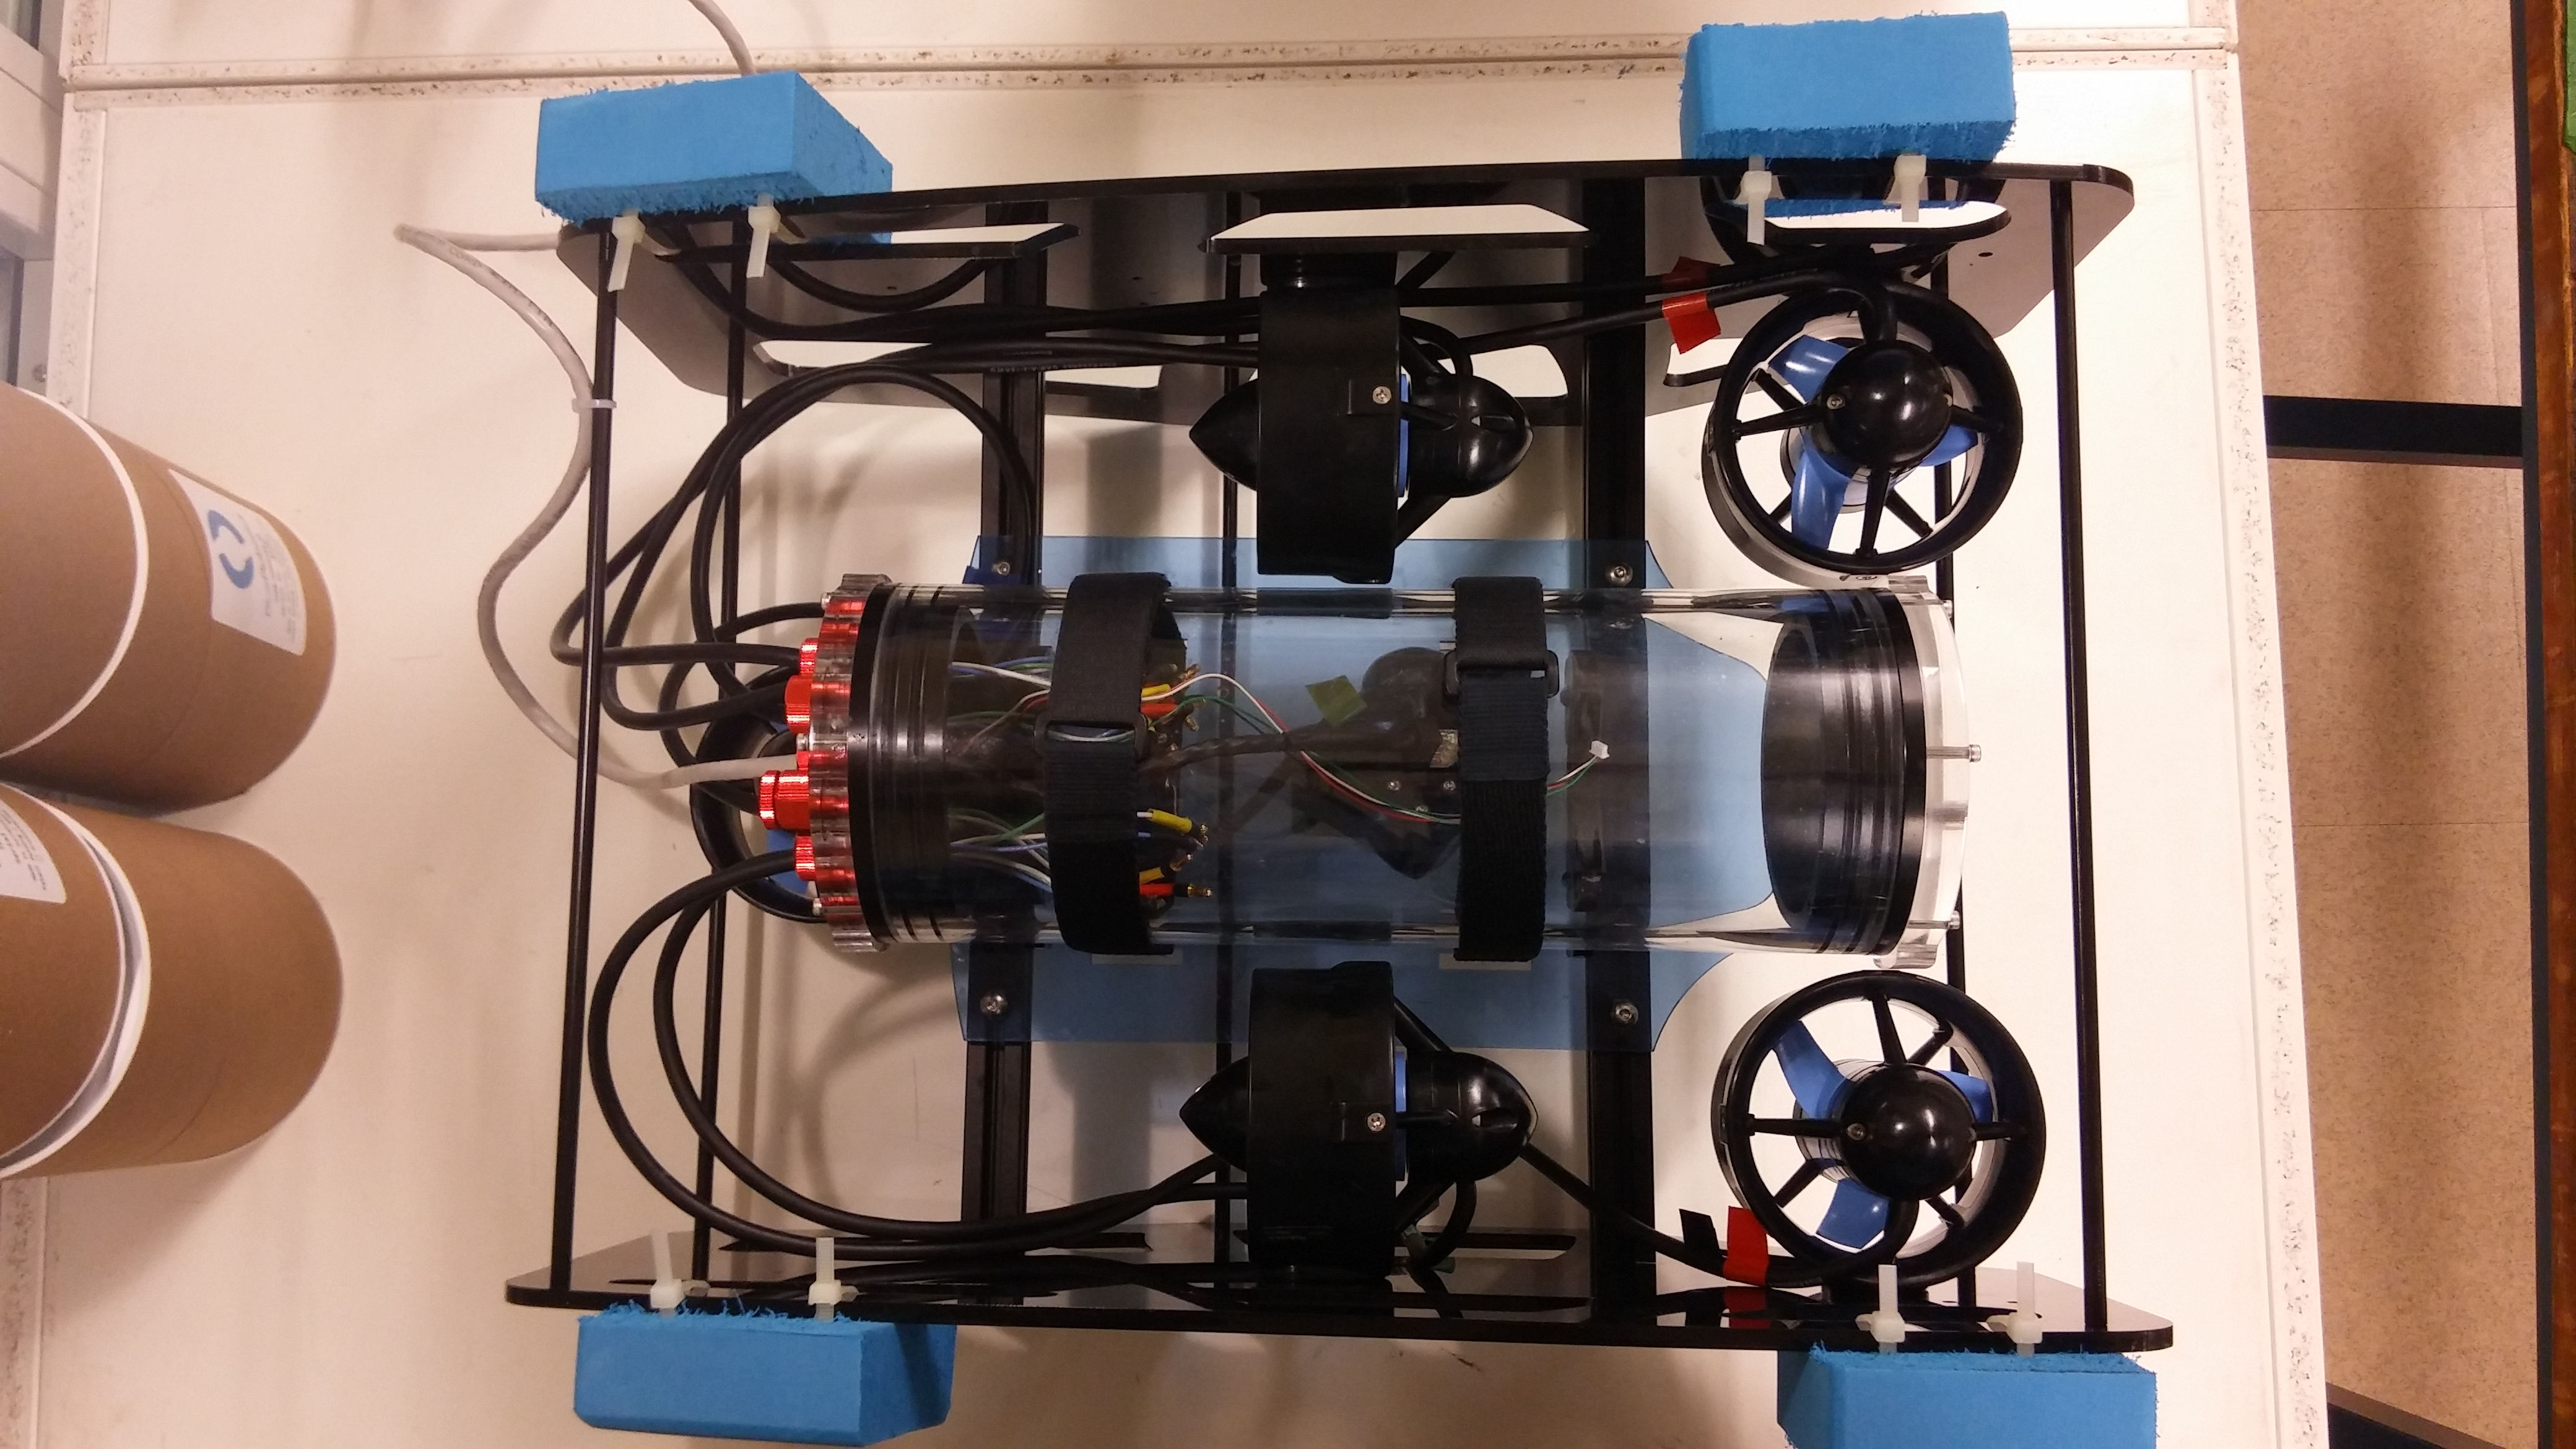
\includegraphics[trim={28cm 0cm 22cm 5cm},clip,width=\textwidth]{fig/thrusterlocationtop}};
    \begin{scope}[x={(image.south east)},y={(image.north west)}]
		\pgfmathsetmacro\coordinateRadius{0.025}
        \pgfmathsetmacro\by{\coordinateRadius*sin(45)}
        \pgfmathsetmacro\bx{\coordinateRadius*cos(45)}
        \pgfmathsetmacro\ay{\coordinateRadius*sin(\coordRot)}
        \pgfmathsetmacro\ax{\coordinateRadius*cos(\coordRot)}
        \pgfmathsetmacro\coordYRot{sin(\coordRot)}
        \pgfmathsetmacro\coordXRot{cos(\coordRot)}
        
        \coordinate (O) at (0.48,0.52);
        \draw[red, ultra thick,->] (O) ++(\coordinateRadius,0) -- ++(0.4,0) node[anchor=north east]{\large\color{red}$\xPosition$};
        \draw[red, ultra thick,->] (O) ++(0,-\coordinateRadius)-- ++(0,-0.4) node[anchor=south east]{\large\color{red}$\yPosition$};
        \draw[red, ultra thick] (O) circle (\coordinateRadius); 
        \draw[red, ultra thick] (O) ++(0,\coordinateRadius) node[above]{\large\color{red}$\zPosition$};
        \draw[red, ultra thick] (O) -- ++(\bx,\by) (O) -- ++(-\bx,-\by) (O) -- ++(-\bx,\by) (O)  -- ++(\bx,-\by);
        
        \draw[yellow, ultra thick, <->] (O) ++(0.34,0) -- ++(0,0.23)  node [midway, left] {\large\distance{y}{1}};
        \draw[red, ultra thick] (O) ++(0.34,0.23) node[right]{\large Thruster 1};
        \draw[yellow, ultra thick, <->] (O) ++(0.34,0) -- ++(0,-0.28) node [midway, left] {\large\distance{y}{2}};
        \draw[red, ultra thick] (O) ++(0.34,-0.28) node[right]{\large Thruster 2};
        \draw[yellow, ultra thick, <->] (O) ++(0.03,0) -- ++(0,0.24)  node [midway, right] {\large\distance{y}{3}};
        \draw[red, ultra thick] (O) ++(0.03,0.24) node[right]{\large Thruster 3};
        \draw[yellow, ultra thick, <->] (O) ++(0.03,0) -- ++(0,-0.28) node [midway, right] {\large\distance{y}{4}};
        \draw[red, ultra thick] (O) ++(0.03,-0.28) node[right]{\large Thruster 4};
        
        \draw[yellow, ultra thick, <->] (O) ++(0,0.27) -- ++(0.34,0)  node [midway, above] {\large\distance{x}{1}};
        \draw[yellow, ultra thick, <->] (O) ++(0,-0.32) -- ++(0.34,0)  node [midway, below] {\large\distance{x}{2}};
        \draw[yellow, ultra thick, <->] (O) -- ++(-0.30,0)  node [midway, below] {\large\distance{x}{5}};
        \draw[red, thick] (O) ++(-0.35,0) node[rotate=90]{\large Thruster 5};
    \end{scope}
 \end{tikzpicture}
\end{figure}
\end{column}

\begin{column}{0.5\textwidth}
\begin{figure}
\centering 
\begin{tikzpicture}
    \node[anchor=south west,inner sep=0] (image) at (0,0) {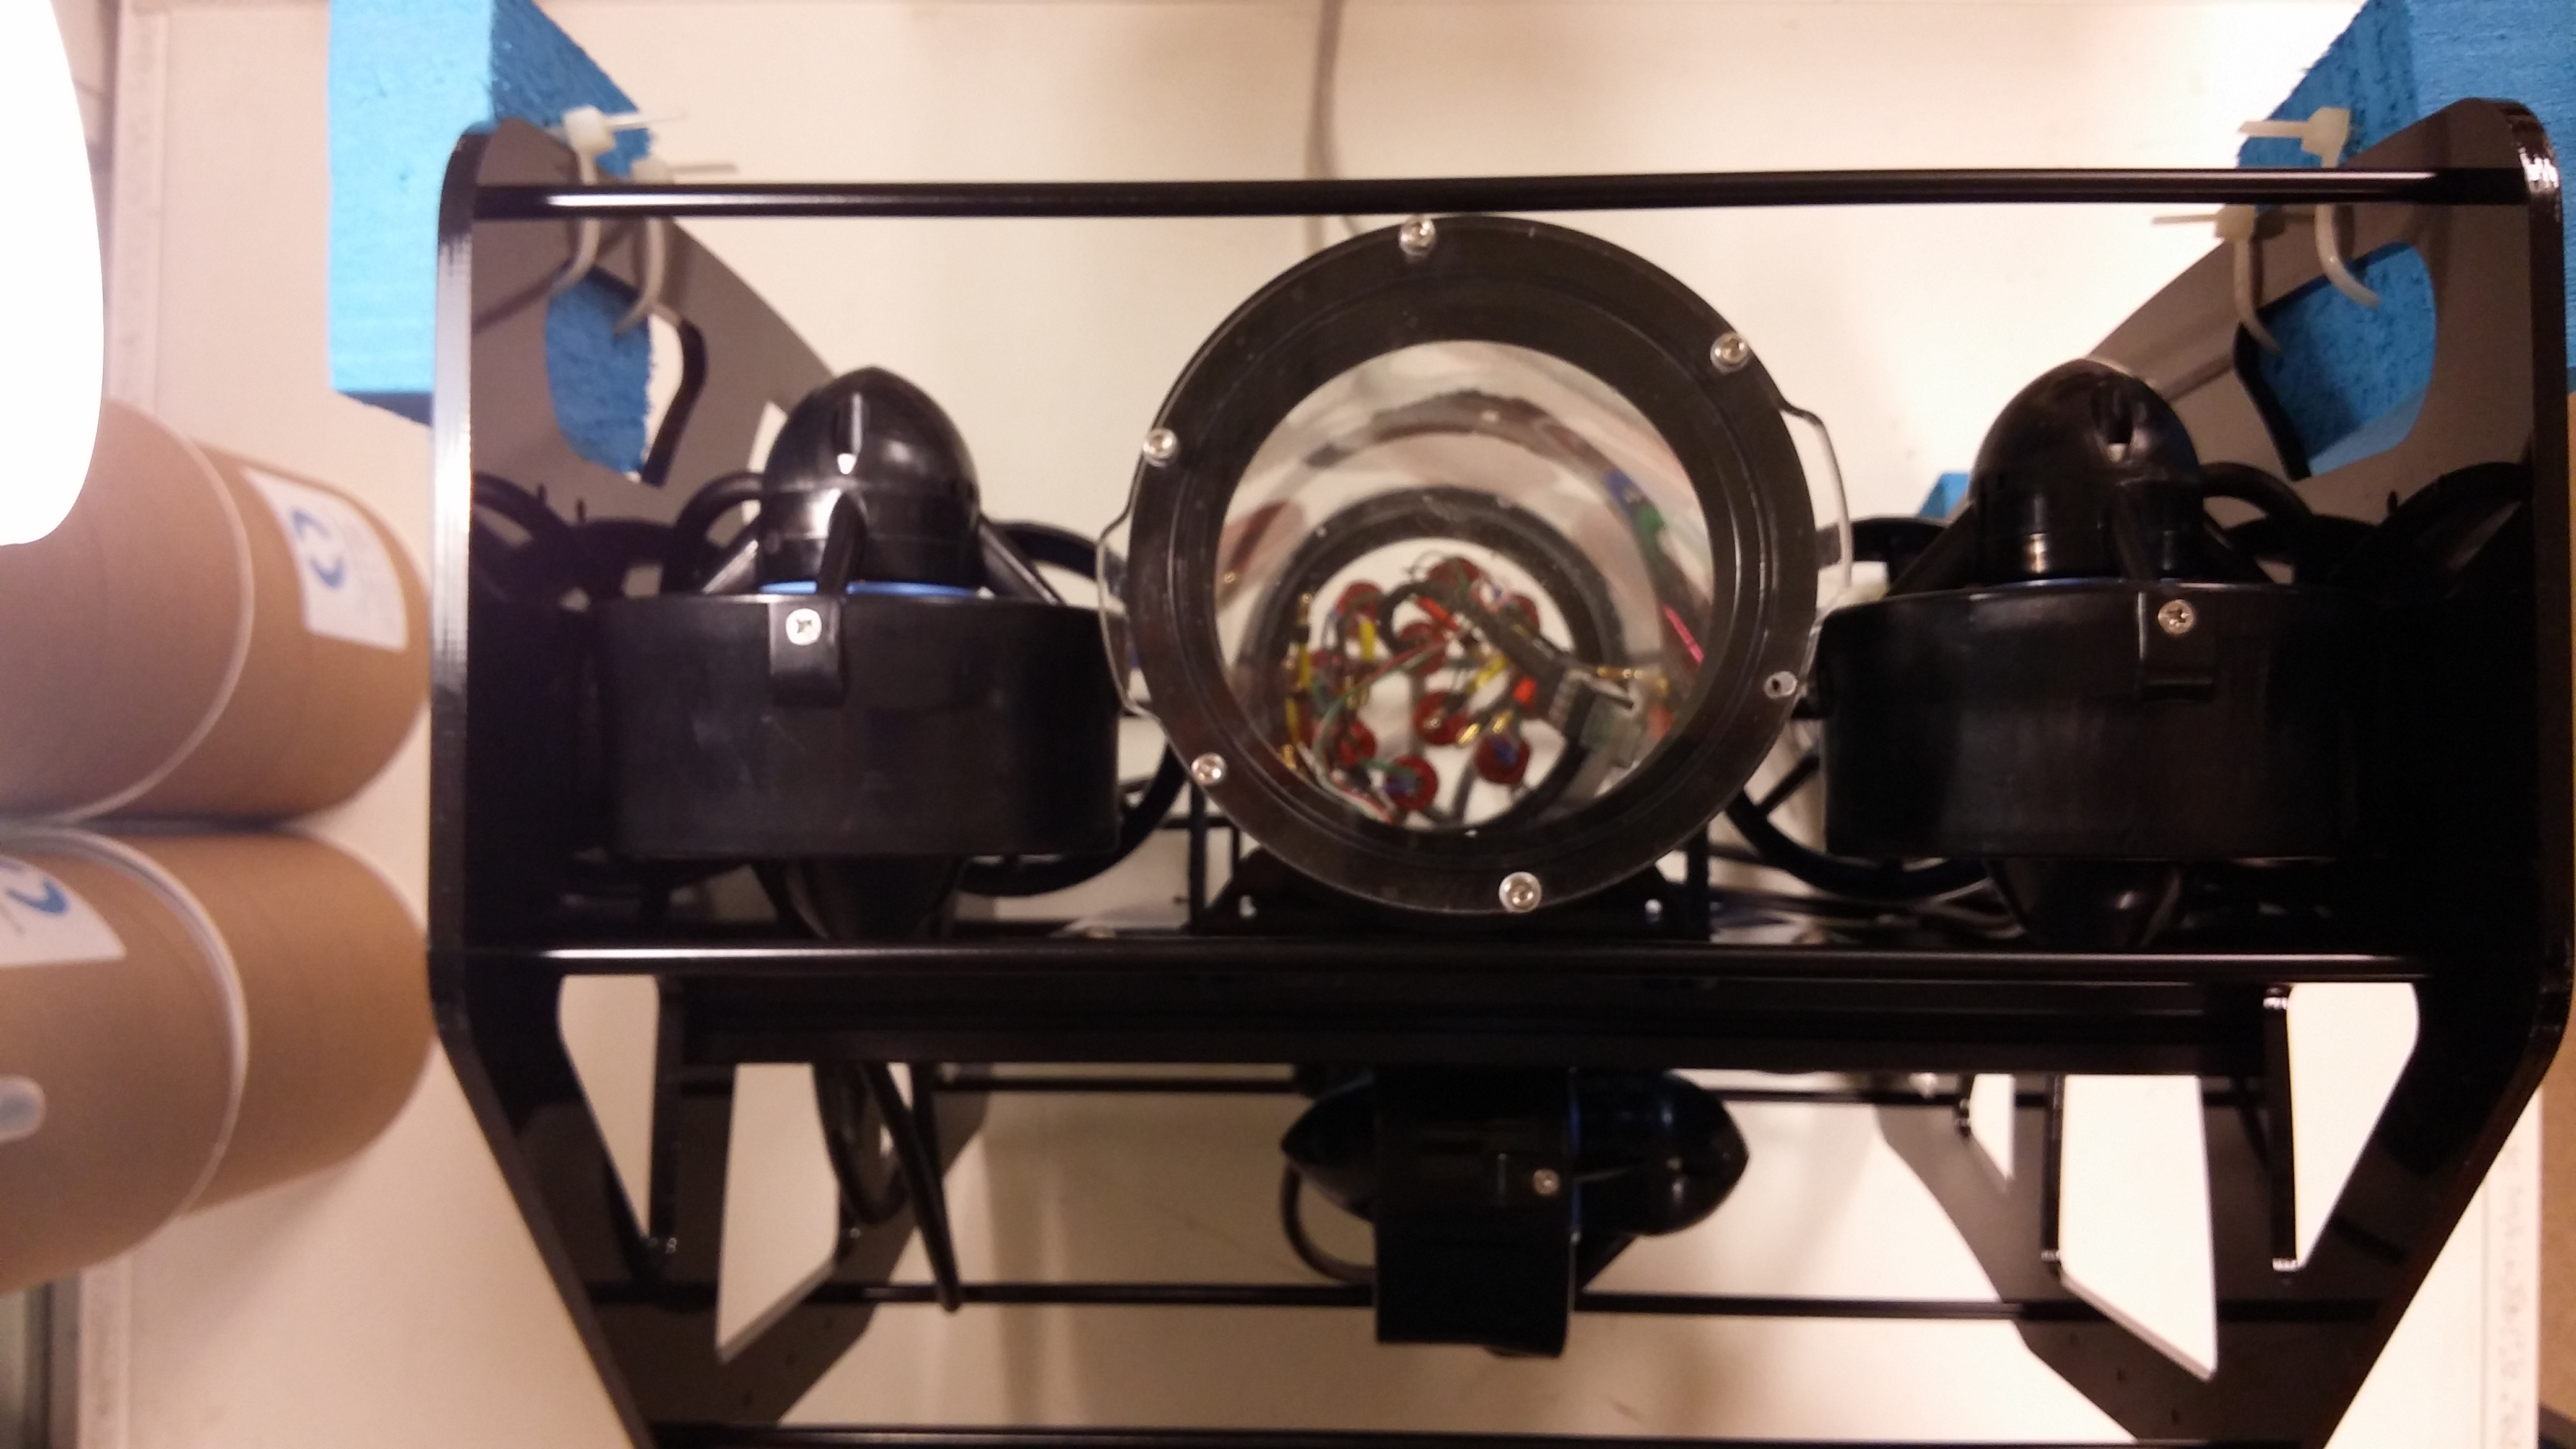
\includegraphics[trim={25cm 2cm 0cm 0cm},clip,width=\textwidth]{fig/thrusterlocationfront}};
    \begin{scope}[x={(image.south east)},y={(image.north west)}]
		\pgfmathsetmacro\coordinateRadius{0.025}
        \pgfmathsetmacro\by{\coordinateRadius*sin(45)}
        \pgfmathsetmacro\bx{\coordinateRadius*cos(45)}
        \pgfmathsetmacro\ay{\coordinateRadius*sin(\coordRot)}
        \pgfmathsetmacro\ax{\coordinateRadius*cos(\coordRot)}
        \pgfmathsetmacro\coordYRot{sin(\coordRot)}
        \pgfmathsetmacro\coordXRot{cos(\coordRot)}
        
        \coordinate (O) at (0.48,0.55);
        \draw[red, ultra thick,->] (O) ++(-\coordinateRadius,0) -- ++(-0.4,0) node[anchor=north east]{\large\color{red}$\yPosition$};
        \draw[red, ultra thick,->] (O) ++(0,-\coordinateRadius)-- ++(0,-0.5) node[anchor=south east]{\large\color{red}$\zPosition$};
        \draw[red, ultra thick] (O) circle (\coordinateRadius);        
        \draw[red, ultra thick] (O) ++(0,\coordinateRadius) node[above]{\large\color{red}$\xPosition$};
		\draw[red, ultra thick] (O) node[circle,fill,inner sep=1pt]{};
        
        \draw[yellow, thick, <->] (O) ++(0.04,0) -- ++(0,-0.37)  node [midway, right]{\large\distance{z}{6}};
        \draw[red, thick] (O) ++(0.04,-0.37) node[right]{\large Thruster 6};
    \end{scope}
\end{tikzpicture}
\end{figure}
\end{column}
\end{columns}
\note{How the body-fixed coordinate system is located in the ROV.}
\end{frame}

\begin{frame}{6-DOF model}
An underwater vehicle can be modelled as 
\begin{align}
\etaVectordot& = \boldsymbol{J}(\etaVector)\nuVector \\
 \inertia \nuVectordot &+ \coriolis(\nuVector)\nuVector + \damping(\nuVector)\nuVector + \gravity(\etaVector) = \tauVector 
\end{align}
\note{\begin{itemize}
\item Equation 1 is the kinematic equations i.e. how the different coordinate systems relate to each other.
\item M is inertia
\item C is Coriolis forces
\item D is damping forces
\item g is gravity and buoyancy
\item $\tau$ are forces and moments
\item Some of these can be divided into hydrostatics, hydrodynamics and rigid-body physics subcomponents.
\end{itemize}}
\end{frame}

\begin{frame}{Rigid-body kinetics}
The rigid-body kinetic relations of the \abbrROV can derived using the Newton-Euler formulation and can be expressed as
\begin{equation}\label{eq:rb}
\inertia_{\text{RB}}\dot{\nuVector} + \coriolis_{\text{RB}}(\nuVector)\nuVector = \tauVector_{\text{RB}}
\end{equation}

The rigid-body inertia matrix
\begin{equation}
   \inertia_{RB} = 
    \begin{bmatrix}
        m\eye{3} & \zero{3} \\
        \zero{3} & \bodyinertia{g}
    \end{bmatrix}
\end{equation}
describes the resistance to change linear and angular velocity.

The Coriolis forces can be described by
\begin{equation}
\begin{split}
    \coriolis_{RB}(\nuVector) &= 
    \begin{bmatrix}
        m\cross{\nuVectorAng}              & -m\cross{\nuVectorAng}\cross{r_g^b}  \\
        m\cross{r_g^b}\cross{\nuVectorAng} & -\cross{\bodyinertia{b}\nuVectorAng} \\
    \end{bmatrix}
\end{split}
\end{equation}
\note{\begin{itemize}
\item Rigid-body kinetics are physical relations derived from Newton-Euler formulations.
\item $I_g$ is the ROV's inertia
\item m is mass
\item Coriolis forces are due to that the ROV travel in a rotating reference frame.
\item S is the vector cross product
\item $r_g^b$ is the distance from the ROV's center of origin to the ROV's center of gravity.
\end{itemize}}
\end{frame}

\begin{frame}{Hydrodynamics}
The forces and affects from interaction with water can be modelled as
\begin{equation} \label{eq:dyn}
 \tauVector_\text{{Dyn}}=-\inertia_{\text{A}} \dot{\nuVector} -\coriolis_{\text{A}}(\nuVector)\nuVector - \damping(\nuVector)\nuVector  
\end{equation} 


The added mass and moment if inertia is defined as
\begin{equation}
\inertia_\text{A} =
-\begin{bmatrix}
    \Xudot & 0 & 0 & 0 & 0 & 0 \\
    0 & \Yvdot & 0 & 0 & 0 & 0 \\
    0 & 0 & \Zwdot & 0 & 0 & 0 \\
    0 & 0 & 0 & \Kpdot& 0 & 0 \\
    0 & 0 & 0 & 0 & \Mqdot & 0 \\
    0 & 0 & 0 & 0 & 0 & \Nrdot \\
    \end{bmatrix}
\end{equation}
under the assumption that the ROV moves at low speeds relative to the water.
\end{frame}

\begin{frame}
The Coriolis-centripetal effects from the added mass and added moment of inertia are described as
\begin{align}
    \coriolis_\text{A}(\nuVector) &= 
    \begin{bmatrix}
    0 & 0 & 0 & 0 & -\Zwdot w & \Yvdot v \\
    0 & 0 & 0 & \Zwdot w & 0 & -\Xudot u \\
    0 & 0 & 0 & -\Yvdot v & \Xudot u & 0 \\
    0 & -\Zwdot w & \Yvdot v & 0 & -\Nrdot r & \Mqdot q \\
    \Zwdot w & 0 & -\Xudot u & \Nrdot r & 0 & -\Kpdot p \\
    -\Yvdot v & \Xudot u & 0 & - \Mqdot q & \Kpdot p & 0 \\
    \end{bmatrix}
\end{align}
under the assumption that the \abbrROV is moving slowly and has three planes of symmetry.
\end{frame}

\begin{frame}
The linear and quadratic hydrodynamic damping can be described as
\begin{align}
\begin{split}
    \damping(\nuVector) &= \\
    -& \scalemath{0.5}{\begin{bmatrix}
        \Xu+\Xuabsu\abs{u} & 0 & 0 & 0 & 0 & 0 \\
        0 & \Yv+\Yvabsv\abs{v} & 0 & 0 & 0 & 0 \\
        0 & 0 & \Zw+\Zwabsw\abs{w} & 0 & 0 & 0 \\
        0 & 0 & 0 & \Kp+\Kpabsp\abs{p} & 0 & 0 \\
        0 & 0 & 0 & 0 & \Mq+\Mqabsq\abs{q} & 0 \\
        0 & 0 & 0 & 0 & 0 & \Nr+\Nrabsr\abs{r} \\
    \end{bmatrix}}
    \end{split}
\end{align}
where it is assumed that the \abbrROV is symmetric about the $xz$-plane and that the damping is decoupled.
\end{frame}

\begin{frame}{Hydrostatics}
The ROV will experience forces and moments caused by the Earths gravitational pull and the buoyancy force the can be modelled as 
\begin{equation}\label{eq:stat}
\tauVector_{\text{Stat}}=-\gravity(\etaVector) = - \begin{bmatrix}
    \boldsymbol{f}_g + \boldsymbol{f}_b \\
    \boldsymbol{r}_b \times \boldsymbol{f}_b + \boldsymbol{r}_g \times \boldsymbol{f}_g 
     \end{bmatrix}
\end{equation} 
\end{frame}

\begin{frame}{Actuators}
The \abbrROV is equipped with six identical, three-bladed thrusters. These can be modelled as
\begin{align}\label{eq:act}
    \scalemath{0.9}{\tauVector_{\text{Act}} =  \thrusterGeometry \boldsymbol{\thrusterfun{}} 
    =
    \begin{bmatrix}
    0& 0& 1& 1& 0& 0\\
    0& 0& 0&  0& 0& -1\\
    -1& -1& 0& 0& -1& 0\\
    \distance{y}{1} & -\distance{y}{2} & 0 &  0 &  0 & \distance{z}{6} \\
    \distance{x}{1} & \distance{x}{2} & 0 & 0 & -\distance{x}{5} & 0 \\
    0 & 0 & \distance{y}{3} & -\distance{y}{4} & 0 & 0 \\
    \end{bmatrix}
    \begin{bmatrix}
    \thrusterfun{1} \\
    \thrusterfun{2} \\
    \thrusterfun{3} \\
    \thrusterfun{4} \\
    \thrusterfun{5} \\
    \thrusterfun{6} \\
    \end{bmatrix}}
\end{align}
\end{frame}

\begin{frame}{Component form}
Using the relation
\begin{equation}
\tauVector_{\text{RB}} = \tauVector_{\text{Dyn}} + \tauVector_{\text{Stat}} + \tauVector_{\text{Act}} + \tauVector_{\text{Dist}}
\end{equation} \eqref{eq:rb}, \eqref{eq:dyn} and \eqref{eq:stat} can be combined to form
\begin{equation}
\scalemath{0.85}{\inertia_{\text{RB}}\dot{\nuVector} + \coriolis_{\text{RB}}(\nuVector)\nuVector + \inertia_{\text{A}} \dot{\nuVector} +\coriolis_{\text{A}}(\nuVector)\nuVector + \damping(\nuVector)\nuVector + \gravity(\etaVector) = \tauVector_\text{{Act}} + \tauVector_{\text{Dist}}}
\end{equation}
This equation can be rearranged to
\begin{equation}
\inertia \dot{\nuVector} + \coriolis(\nuVector)\nuVector + \damping(\nuVector)\nuVector + \gravity(\etaVector) = \tauVector_{\text{Act}} + \tauVector_{\text{Dist}} \approx \tauVector_{\text{Act}}
\end{equation}
where $\inertia = \inertia_{\text{RB}} + \inertia_{\text{A}}$ and $\coriolis(\nuVector)=\coriolis_{\text{RB}}(\nuVector)+\coriolis_{\text{A}}(\nuVector)$.
The expression can then be solved for $\nuVectordot$ and split into components 

\end{frame}

\begin{frame}[shrink]
Data-collection experiments can be designed such that linear velocities will be small and thus can linear velocities be neglected
%\begin{subequations}\label{eq:angVelDynamics}
\begin{multline*}
\dot{p} = \frac{\thrusterfun{1} \distance{y}{1} - \thrusterfun{2} \distance{y}{2} + \thrusterfun{6} \distance{z}{6}}{\Ix - \Kpdot} + \frac{ (\Kp + \Kpabsp \abs{p})p}{\Ix - \Kpdot}  + \frac{-\Mqdot q r}{\Ix - \Kpdot} +  \frac{\Nrdot q r}{\Ix - \Kpdot}  + \frac{q r (\Iy - \Iz)}{\Ix - \Kpdot} \\{\color{red} + \frac{- \Yvdot v w}{\Ix - \Kpdot} + \frac{\Zwdot v w}{\Ix - \Kpdot}} + \frac{B z_B \cos{\theta} \sin{\phi}}{\Ix - \Kpdot}
\end{multline*}
\begin{multline*}
\dot{q} =\frac{\thrusterfun{1} \distance{x}{1} + \thrusterfun{2} \distance{x}{2} - \thrusterfun{5} \distance{x}{5}}{\Iy - \Mqdot} + \frac{(\Mq + \Mqabsq \abs{q})q}{\Iy - \Mqdot} + \frac{\Kpdot p r}{\Iy - \Mqdot} + \frac{-\Nrdot p r}{\Iy - \Mqdot}  +
\frac{p r (\Iz - \Ix)}{\Iy - \Mqdot} \\ {\color{red} + \frac{-\Zwdot u w}{\Iy - \Mqdot} + \frac{\Xudot u w}{\Iy - \Mqdot}} + \frac{B z_B \sin{\theta} }{\Iy - \Mqdot} 
\end{multline*}
\begin{multline*}
\dot{r} = \frac{\thrusterfun{3} \distance{y}{3} - \thrusterfun{4} \distance{y}{4}}{\Iz - \Nrdot} + \frac{(\Nr + \Nrabsr \abs{r})r}{\Iz - \Nrdot} + \frac{-\Kpdot p q}{\Iz - \Nrdot} + \frac{\Mqdot p q}{\Iz - \Nrdot} + \frac{p q (\Ix - \Iy)}{\Iz - \Nrdot}\\ {\color{red} + \frac{- \Xudot u v}{\Iz - \Nrdot} + \frac{\Yvdot u v}{\Iz - \Nrdot}}
\end{multline*}
%\end{subequations}
\end{frame}

\begin{frame}[shrink]
To gain identifiability, the reparametrisation $A_p = \Ix - \Kpdot$, $B_q = \Iy - \Mqdot$ and $C_r = \Iz - \Nrdot$ was introduced. These changes resulted in
\begin{subequations}\label{eq:quatModel}
\begin{multline} \label{eq:p_dotWithoutTranslation}
\pdot = \frac{\thrusterfun{1} \distance{y}{1} - \thrusterfun{2} \distance{y}{2} + \thrusterfun{6} \distance{z}{6}}{A_p} + \frac{B z_B \cos{\theta} \sin{\phi}}{A_p} + \frac{(\Kp + \Kpabsp \abs{p})p}{A_p} + \frac{q r (B_q - C_r)}{A_p},
\end{multline}
\begin{multline} \label{eq:q_dotWithoutTranslation}
\qdot = \frac{\thrusterfun{1} \distance{x}{1} + \thrusterfun{2} \distance{x}{2} - \thrusterfun{5} \distance{x}{5}}{B_q} - \frac{B z_B \sin{\theta}}{B_q} + \frac{(\Mq + \Mqabsq \abs{q})q}{B_q} - \frac{p r (A_p - C_r)}{B_q}
\end{multline}
and
\begin{multline} \label{eq:r_dotWithoutTranslation}
\rdot = \frac{\thrusterfun{3} \distance{y}{3} - \thrusterfun{4} \distance{y}{4}}{C_r} + \frac{(\Nr + \Nrabsr \abs{r})r}{C_r} + \frac{p q (A_p  - B_q)}{C_r}
\end{multline}
\end{subequations}
\end{frame}


\begin{frame}[shrink]
\begin{subequations} \label{eq:pq_dot_decouple}
\begin{multline} \label{eq:pq_dot_decouple1}
\pdot = \frac{\thrusterfun{1} \distance{y}{1} - \thrusterfun{2} \distance{y}{2} + \thrusterfun{6} \distance{z}{6}}{A_p} + \frac{(Kp + \Kpabsp \abs{p})p}{A_p} + \frac{B z_B \cos{\theta} \sin{\phi}}{A_p},
\end{multline}  
\begin{multline} \label{eq:pq_dot_decouple2}
\qdot =\frac{\thrusterfun{1} \distance{x}{1} + \thrusterfun{2} \distance{x}{2} - \thrusterfun{5} \distance{x}{5}}{B_q} + \frac{(\Mq + \Mqabsq \abs{q})q}{B_q} + \frac{B z_B \sin{\theta}}{B_q} 
\end{multline}  
\end{subequations} and
\begin{equation} \label{eq:r_dot_decouple}
\rdot = \frac{\thrusterfun{3} \distance{y}{3} - \thrusterfun{4} \distance{y}{4}}{B_q} + \frac{(\Nr + \Nrabsr \abs{r})r}{B_q}
\end{equation}
\note{qwe}
\end{frame}

%%%%%%%%%%%%%%%%%%%%%Parameter Estimation%%%%%%%%%%%%%%%%%%%%%%%%%%%%%%%%%%%%%%%%%%%%%%%%%%%%%%%%%%%%%%%%%%
\section{Parameter Estimation}
\begin{frame}
What is parameter estimation and why is it needed
pem and problems
kalman smoother
pem results
kalman estimation
kalman results
discussion
\end{frame}

%%%%%%%%%%%%%%%%%%%%%Controllers%%%%%%%%%%%%%%%%%%%%%%%%%%%%%%%%%%%%%%%%%%%%%%%%%%%%%%%%%%%%%%%%%%

\section{Controllers}
\begin{frame}
\begin{columns}
\begin{column}{0.5\textwidth}
\begin{itemize}
\item  \structure<1> {What is automatic control}
\item  \structure<2>{Open-loop control}
\item  \structure<3>{Feed-back control}
\item  \structure<4->{Exact linearisation}
\end{itemize}
\end{column}
\begin{column}{0.5\textwidth}
\only<2-2>{
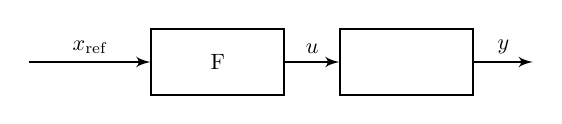
\begin{tikzpicture}[auto, scale=0.8, every node/.style={scale=0.8}, thick, node distance=2cm,>=latex',
 block/.style  = {draw, rectangle,minimum height=3em, minimum width=6em},
 sum/.style    = {draw, circle, inner sep=0pt, text width=4mm,align=center, node distance=1cm},
 input/.style  = {coordinate},
 output/.style = {coordinate},
 pinstyle/.style = {pin edge={to-,thin,black}}]
 
 \node [input, name=input] {};
 \node [block, right of=input, node distance=3cm] (controller) {F};
 \node [block, right of=controller, node distance=3cm] (system) {\abbrROV};

 \draw [->] (controller) -- node[name=u] {$u$} (system);
 \node [output, right of=system] (output) {};

 \draw [draw,->] (input) -- node {$x_{\text{ref}}$} (controller);
 \draw [->] (system) -- node [name=y] {$y$}(output);
\end{tikzpicture}
}
\only<3-3>{
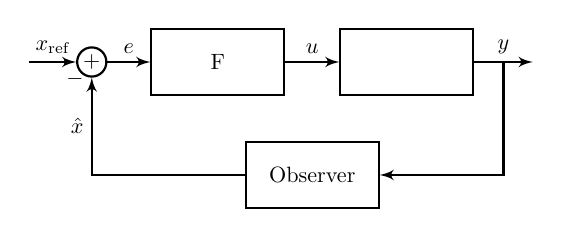
\begin{tikzpicture}[auto, scale=0.8, every node/.style={scale=0.8}, thick, node distance=2cm,>=latex',
			 block/.style  = {draw, rectangle,minimum height=3em, minimum width=6em},
			 sum/.style    = {draw, circle, inner sep=0pt, text width=4mm,align=center, node distance=1cm},
			 input/.style  = {coordinate},
			 output/.style = {coordinate},
			 pinstyle/.style = {pin edge={to-,thin,black}}]
			 
		    \node [input, name=input] {};
		    \node [sum, right of=input] (sum) {+};
		    \node [block, right of=sum] (controller) {F};
		    \node [block, right of=controller, node distance=3cm] (system) {\abbrROV};
		
		    \draw [->] (controller) -- node[name=u] {$u$} (system);
		    \node [output, right of=system] (output) {};
		    \node [block, below of=u] (sensorfusion) {Observer};
		
		    \draw [draw,->] (input) -- node {$x_{\text{ref}}$} (sum);
		    \draw [->] (sum) -- node {$e$} (controller);
		    \draw [->] (system) -- node [name=y] {$y$}(output);
		    \draw [->] (y) |- (sensorfusion);
		    \draw [->] (sensorfusion) -| node[pos=0.99] {$-$} 
		        node [near end] {$\hat{x}$} (sum);
		\end{tikzpicture}
}

\only<4->{
\begin{center}
\begin{align*}
\onslide<5->{
\begin{bmatrix}
\dot{x}_1\\
\dot{x}_2
\end{bmatrix}&=
\begin{bmatrix}
x_2\\
-a x_1 - b x_2\abs{x_2} + u
\end{bmatrix}\\}
%
%
\onslide<6->{
u &= a x_1 +b x_2\abs{x_2} + \bar{u}\\}
%
%
\onslide<7->{
\begin{bmatrix}
\dot{x}_1\\
\dot{x}_2
\end{bmatrix}&=
\begin{bmatrix}
x_2\\
\bar{u}
\end{bmatrix}}
\end{align*}
\end{center}
}
\end{column}
\end{columns}
\note{To control a system towards a desired state using input}
\note{To control the system without measuring the current state. Needs to be modelled in order to attain good performance.}
\note{To base the control action on measurements from outputs of the system.}
\note{To compensate for a systems non-linearities using a model of the system.}
\end{frame}
%what is automatic control
%open-loop control
%exact linearisation
%attitude 
%angular velocity
%depth 
%results
%discussion

\begin{frame}
\begin{center}
Attitude controller using exact linearisation.
\end{center}
\note{An attitude controller has been developed using the exact linearisation technique described earlier.}
\end{frame}
\begin{frame}
\begin{center}
Attitude controller using feedback linearisation
\only<1-1>{
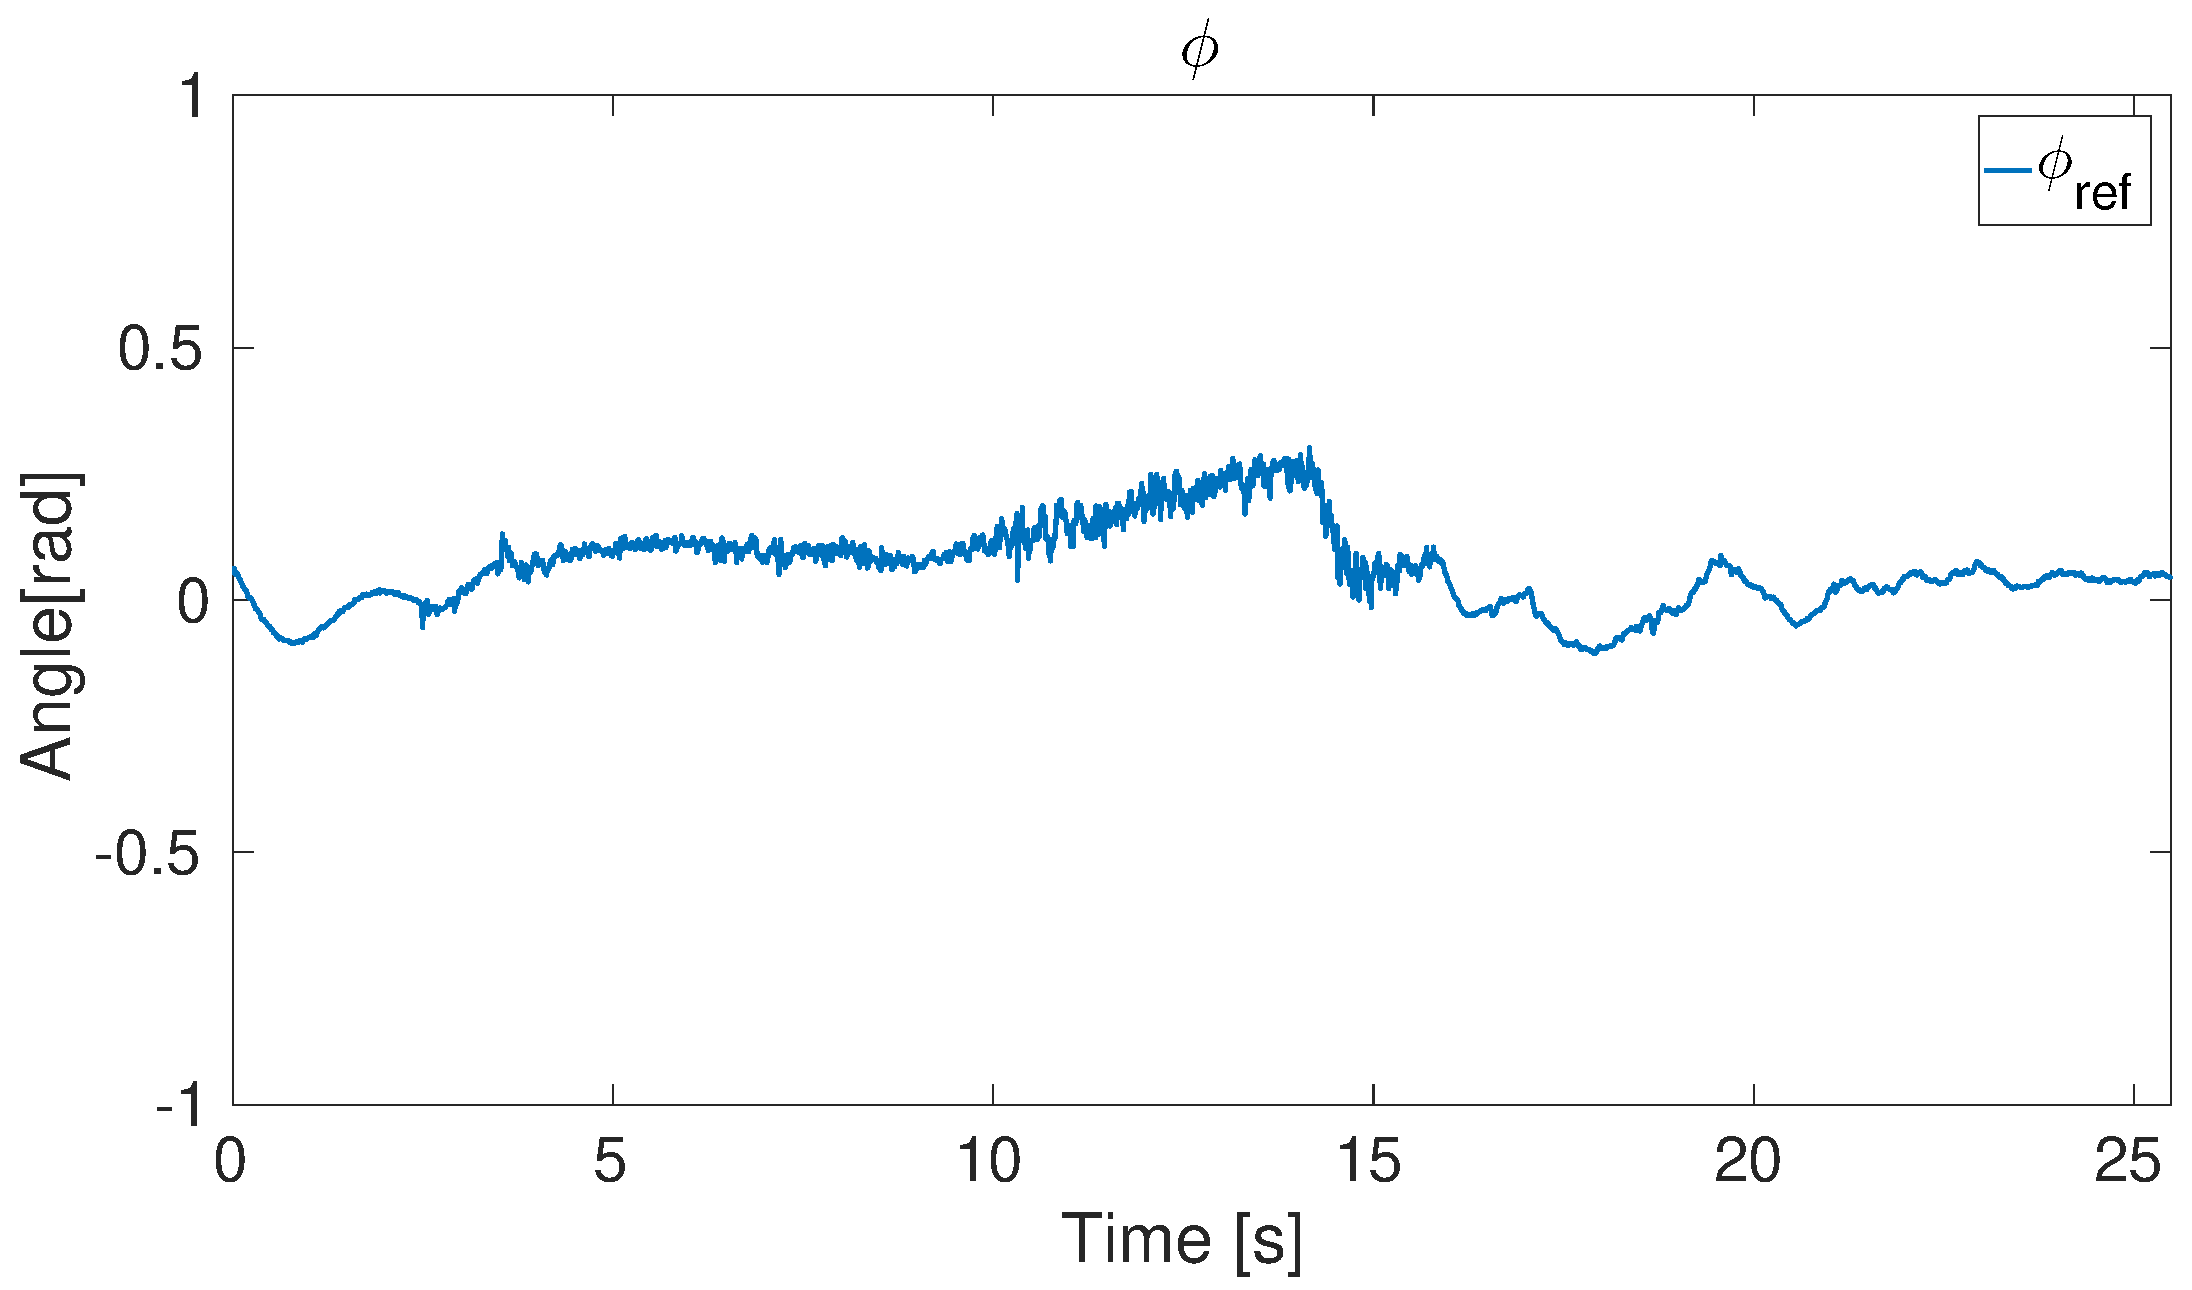
\includegraphics[scale=0.28]{../Master/fig/testExactLinAttitudePhi}
}
\only<2-2>{
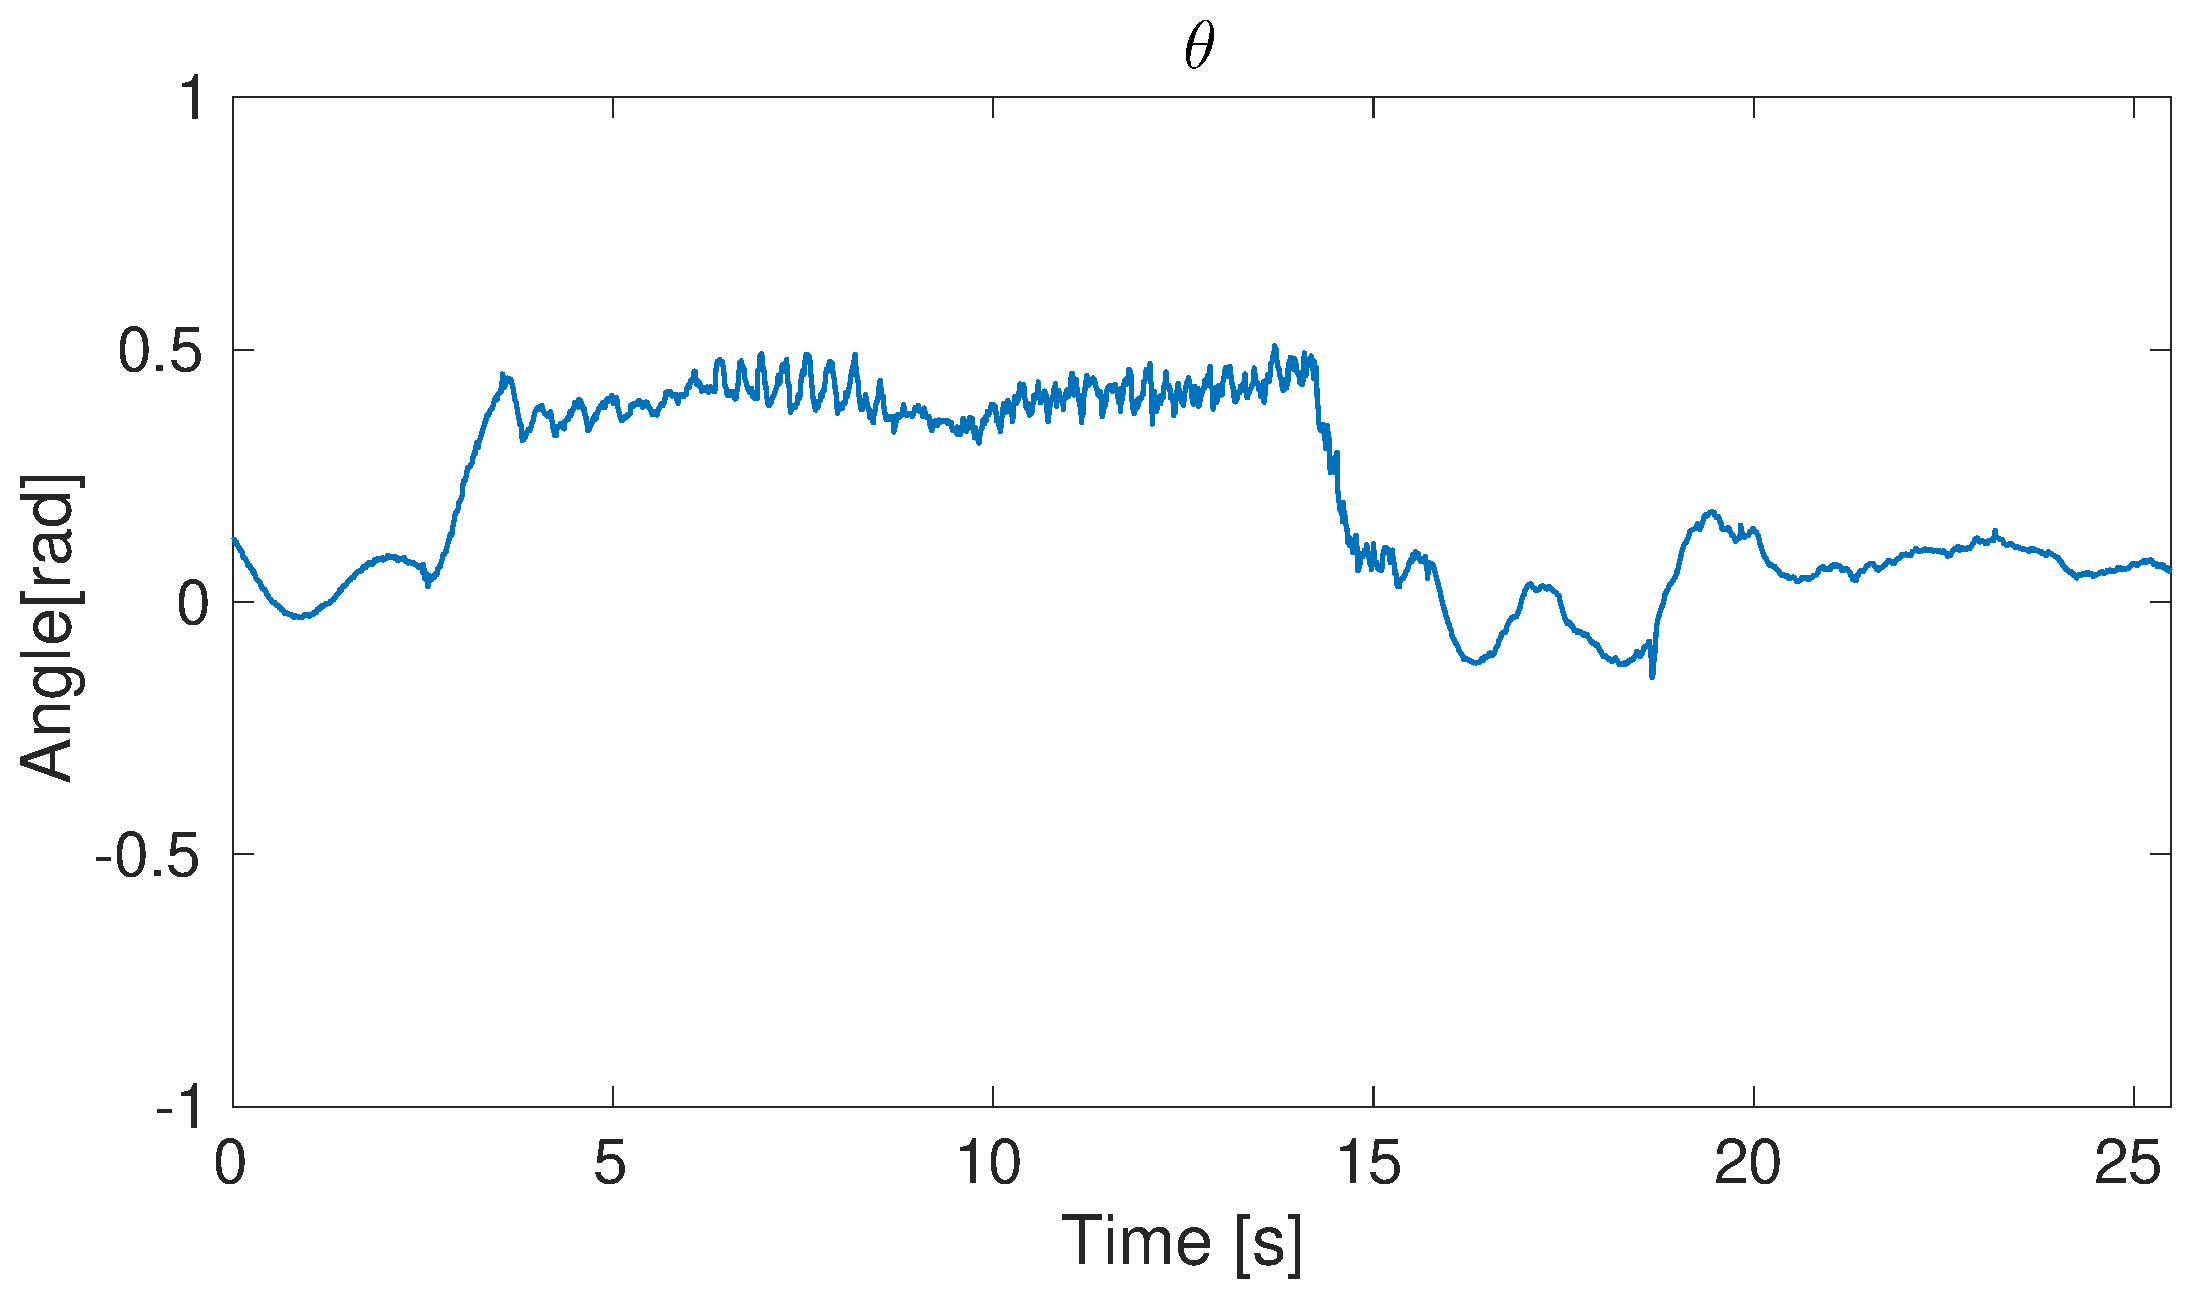
\includegraphics[scale=0.28]{../Master/fig/testExactLinAttitudeTheta}
}
\only<3-3>{
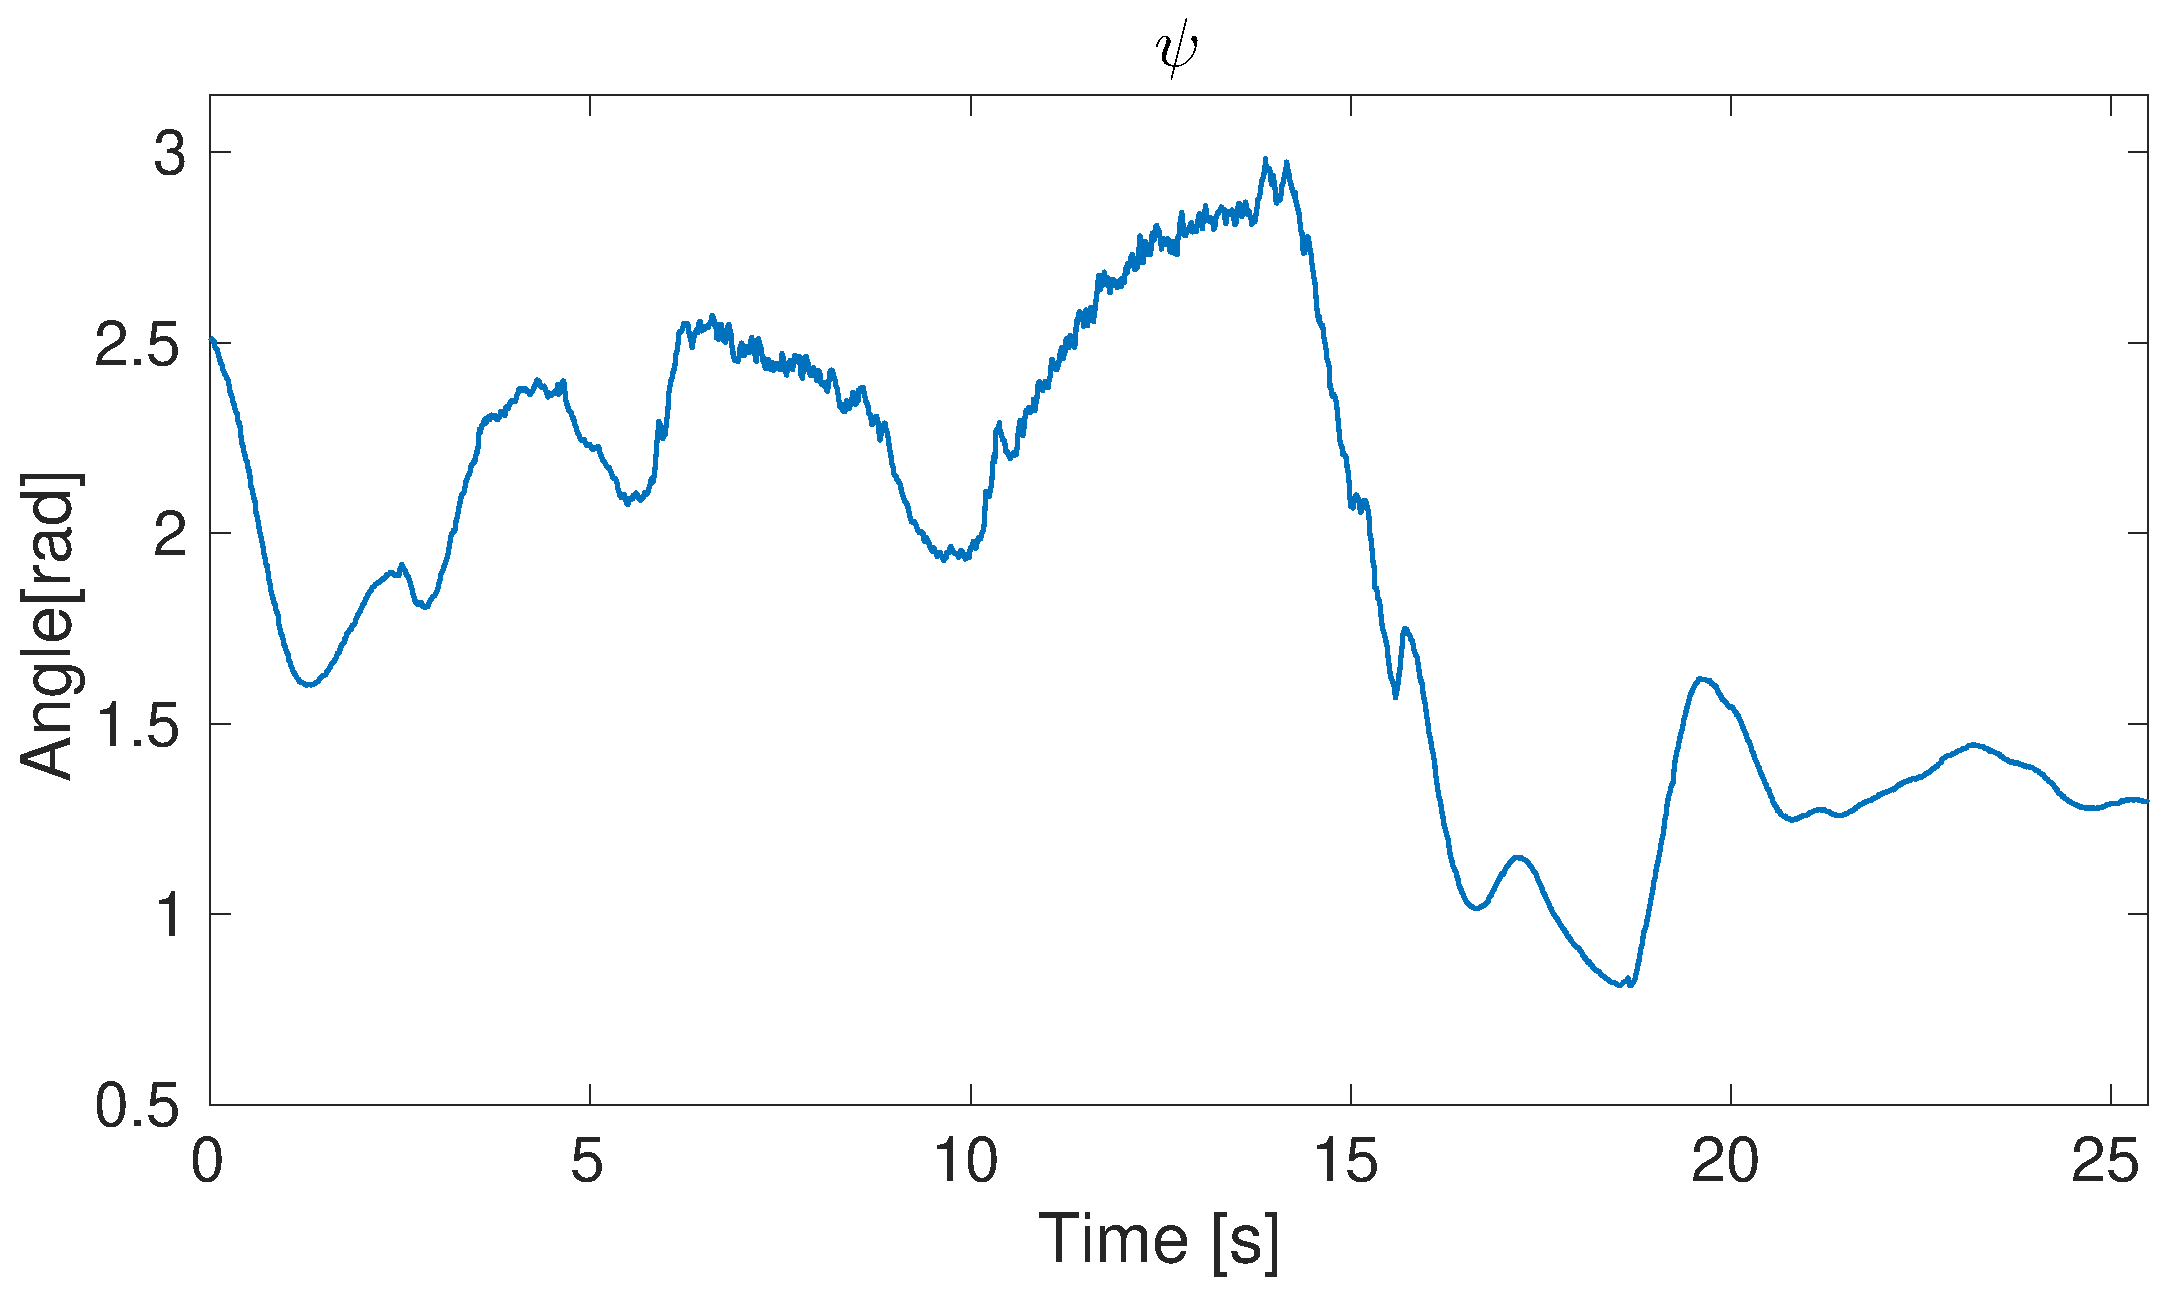
\includegraphics[scale=0.28]{../Master/fig/testExactLinAttitudePsi}
}
\end{center}
\end{frame}
\begin{frame}

\begin{center}
Attitude controller \textbf{without} exact linearisation.

\end{center}
\note{An attitude controller has been developed using the exact linearisation technique described earlier.}
\end{frame}


\begin{frame}
\only<1-1>{
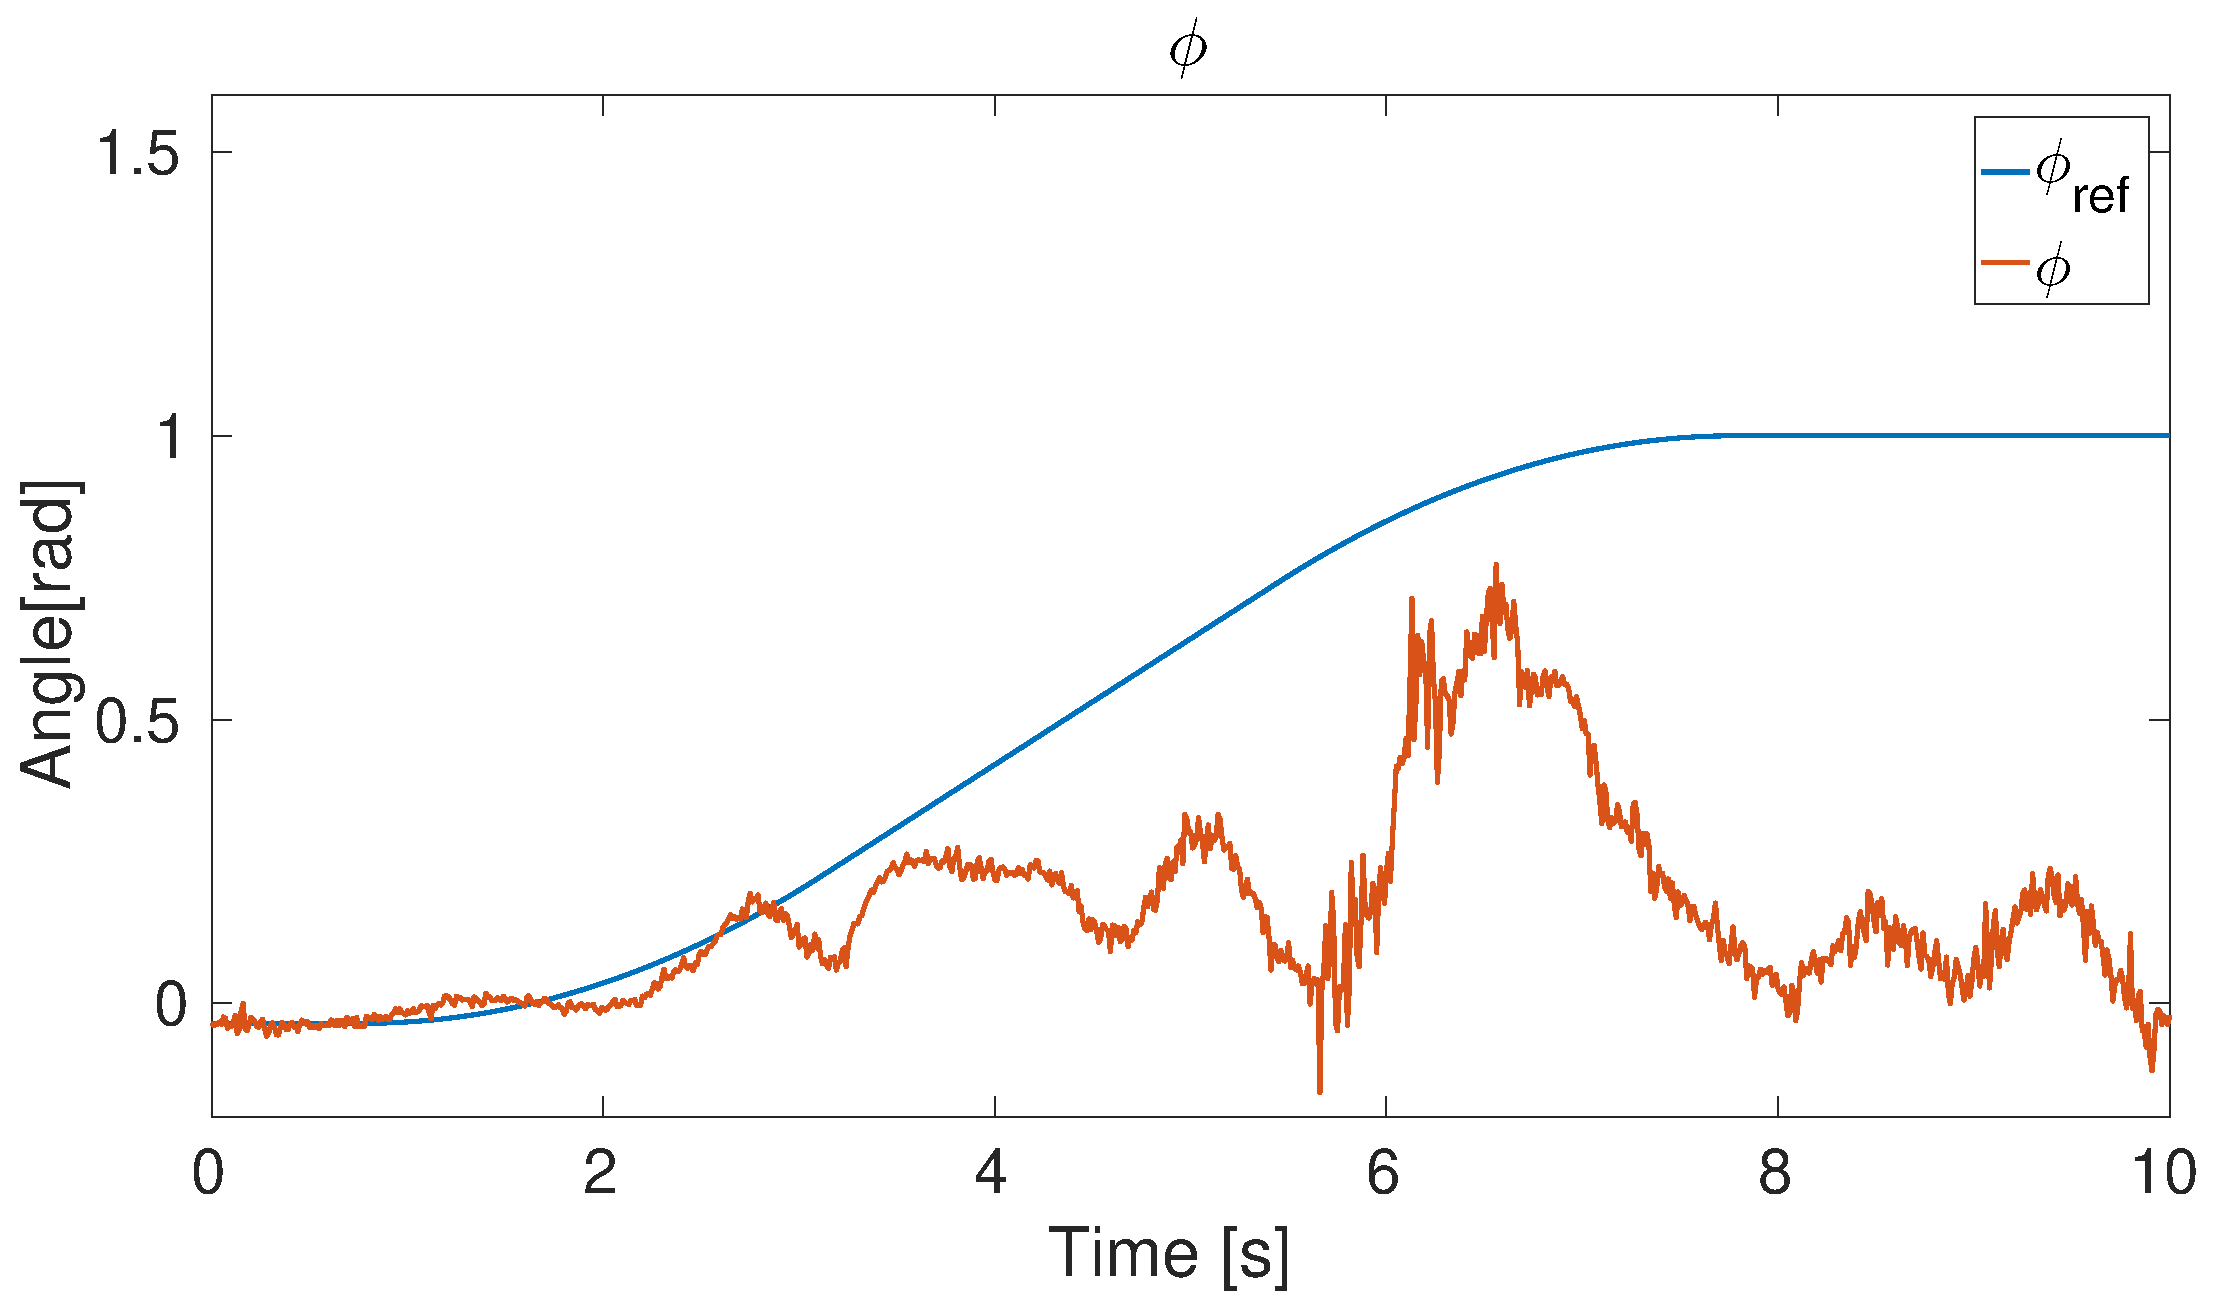
\includegraphics[scale=0.28]{../Master/fig/testStepAllPhis3e10a1}
}
\only<2-2>{
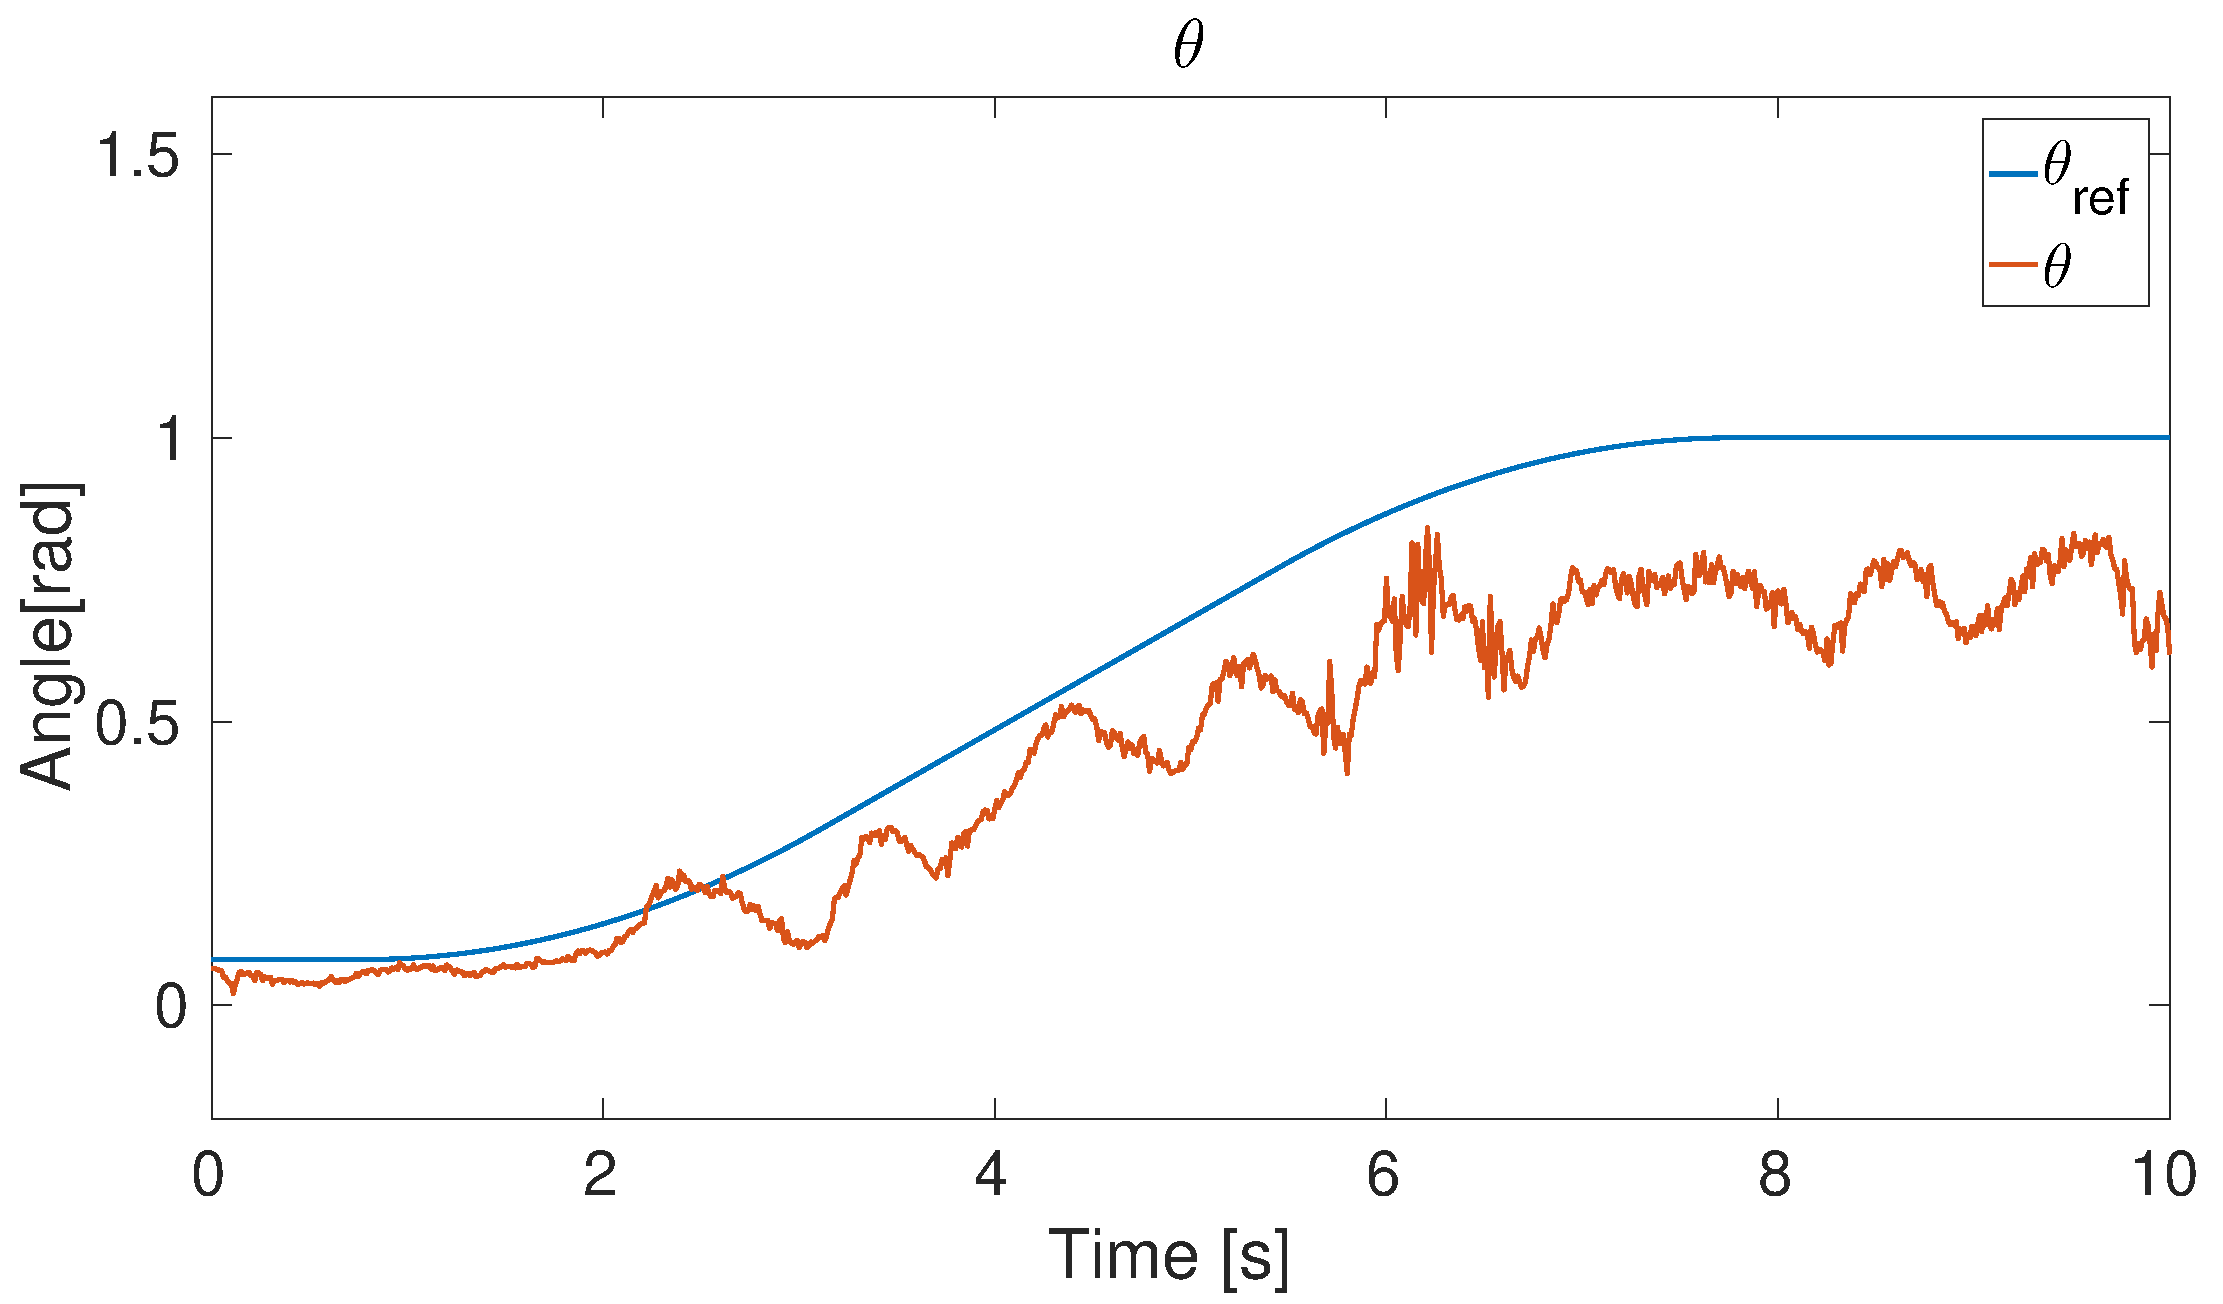
\includegraphics[scale=0.28]{../Master/fig/testStepAllThetas3e10a1}
}
\only<3-3>{
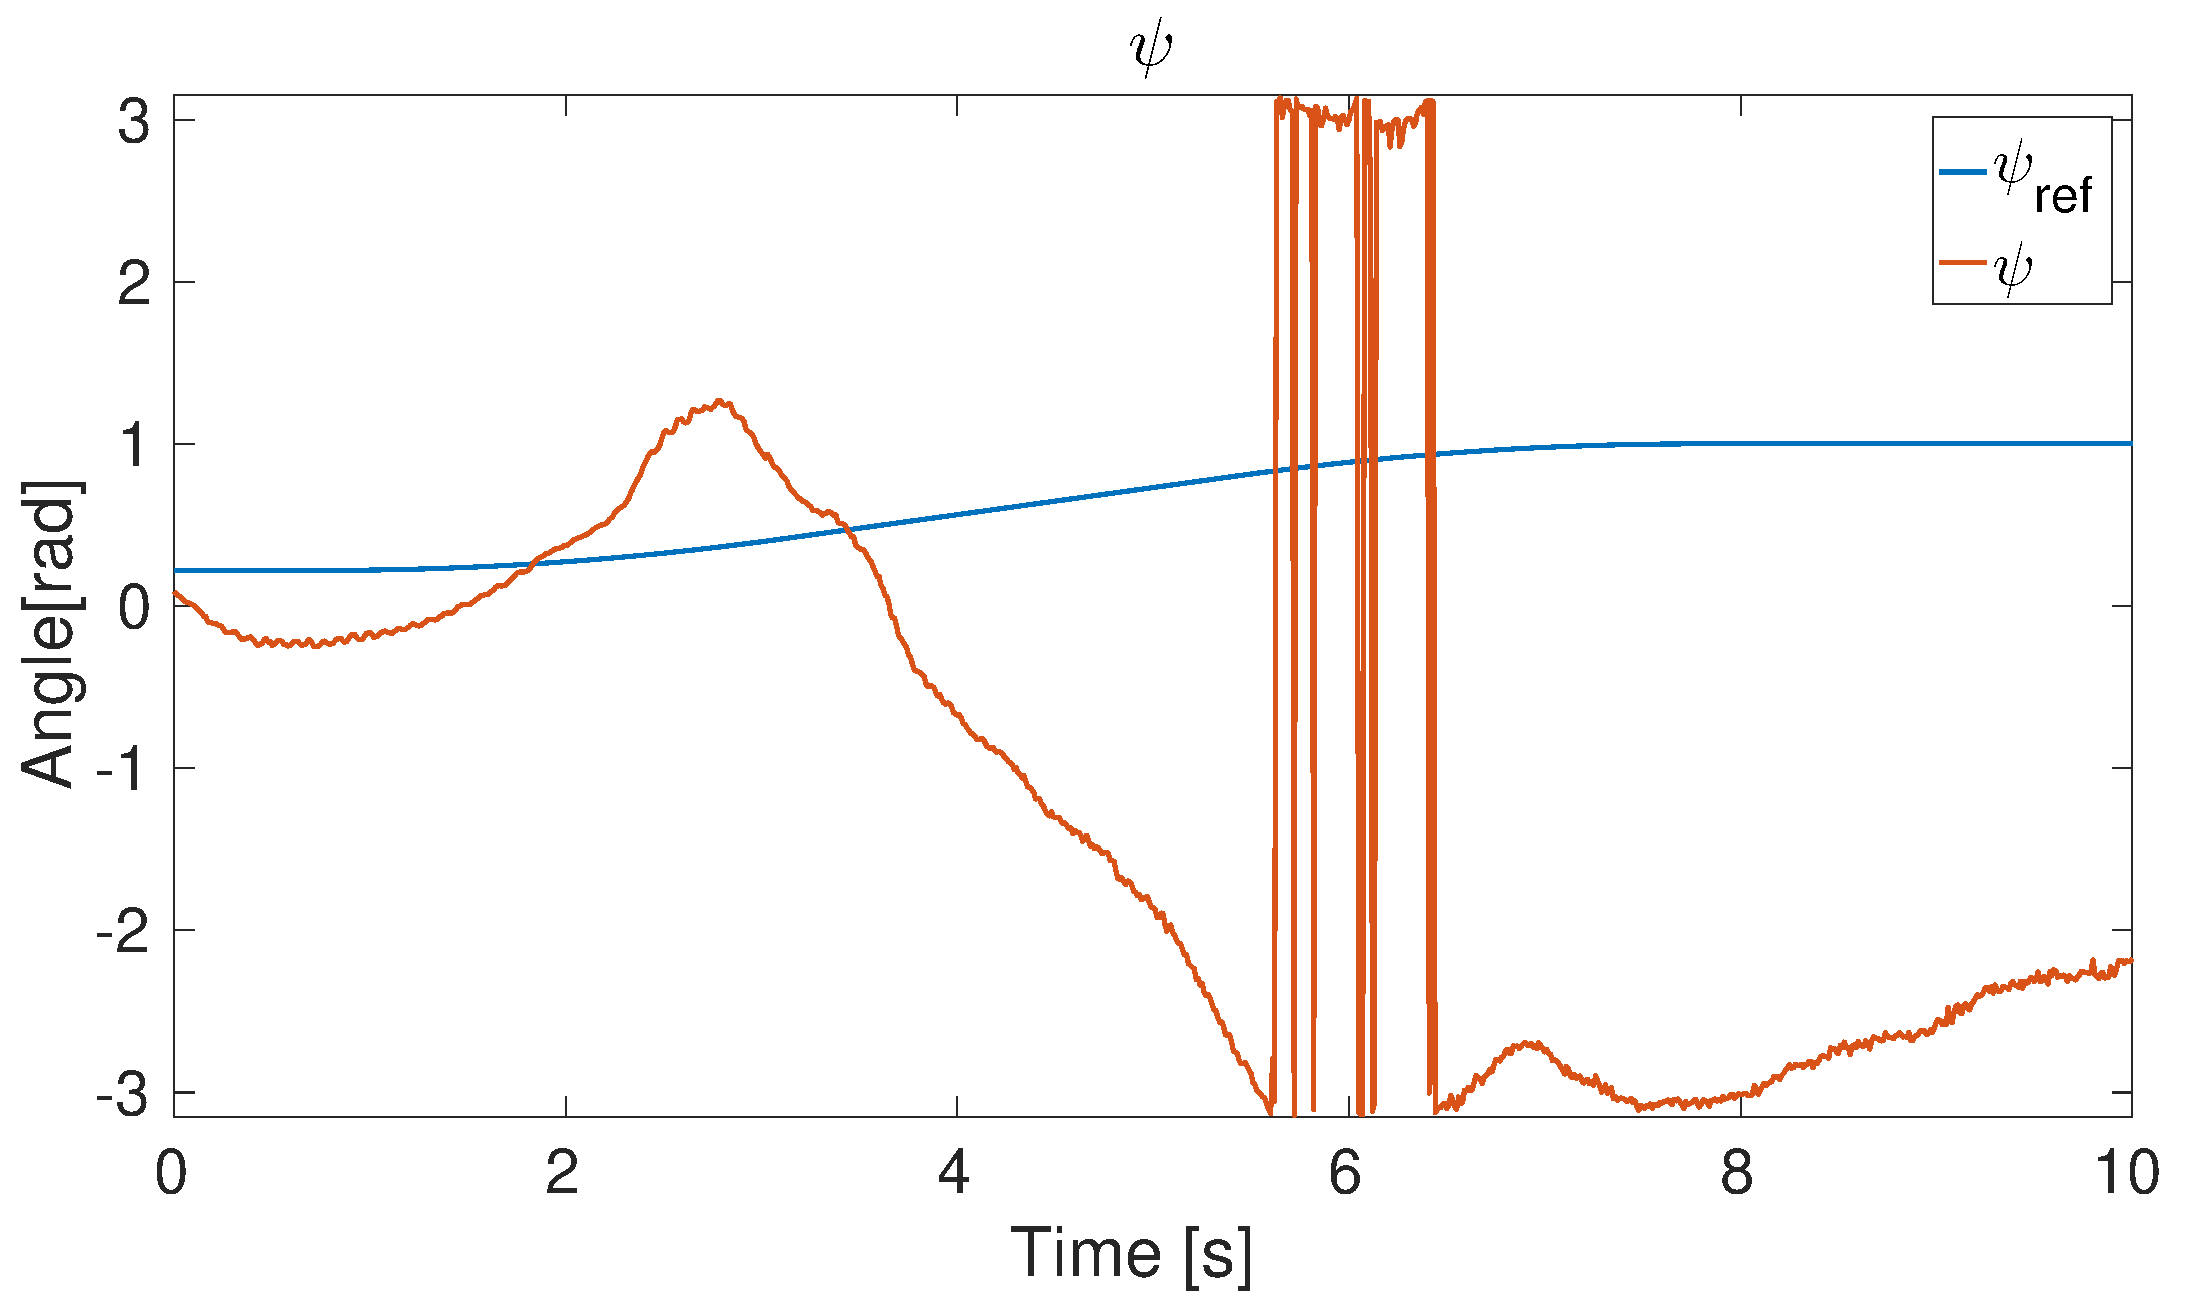
\includegraphics[scale=0.28]{../Master/fig/testStepAllPsis3e10a1}
}
\end{frame}

\begin{frame}
\only<1-1>{
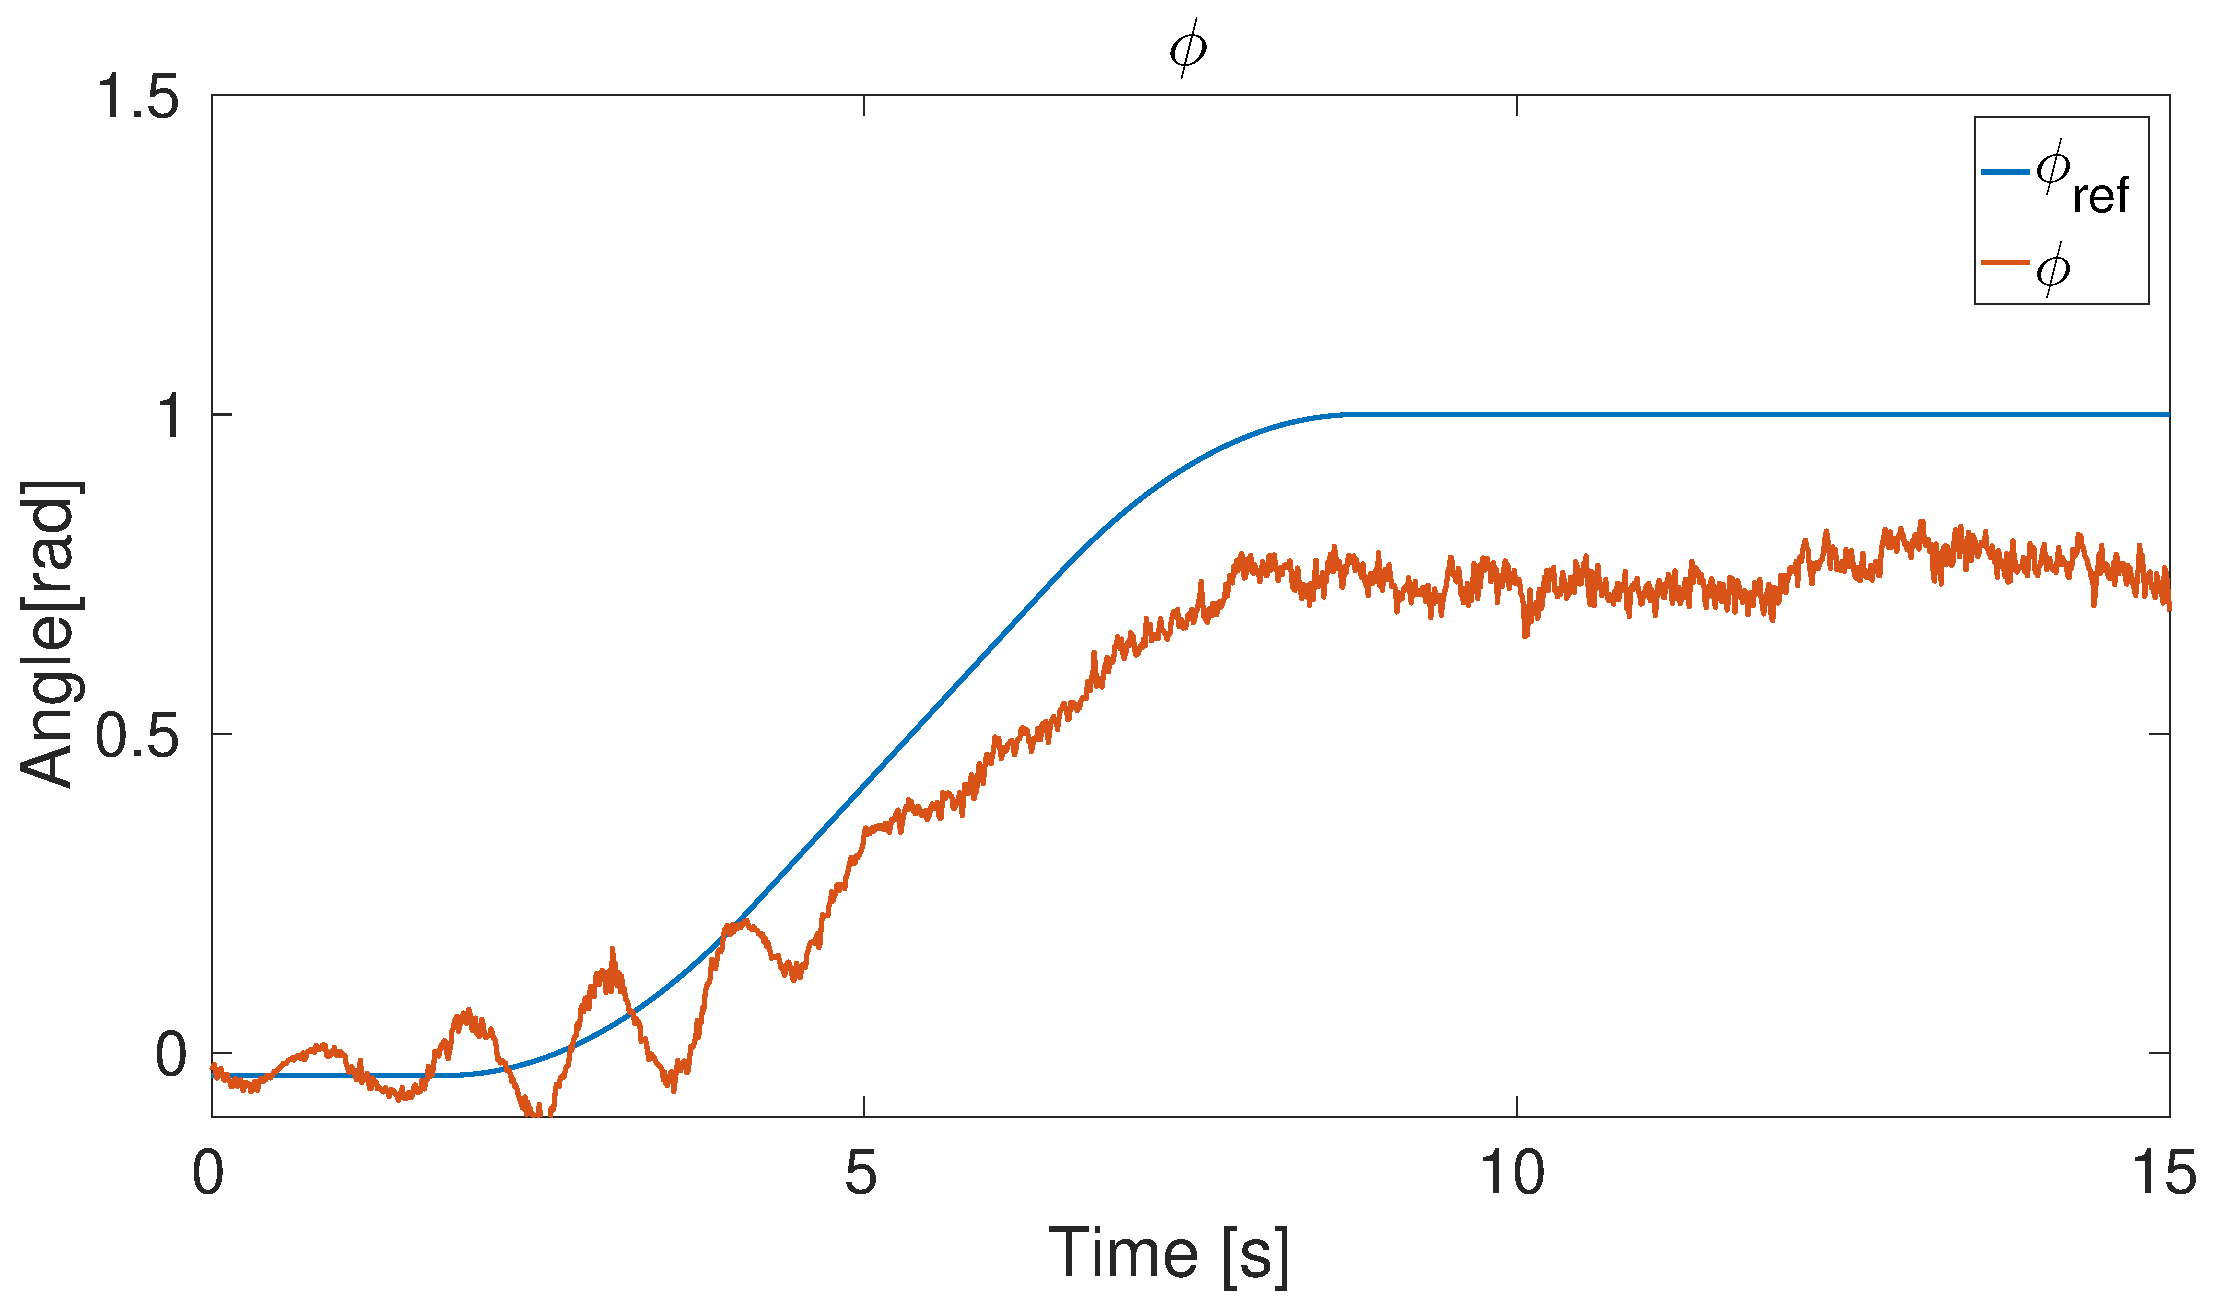
\includegraphics[scale=0.28]{../Master/fig/testStepThetaPhiPhis3e10a1}
}
\only<2-2>{
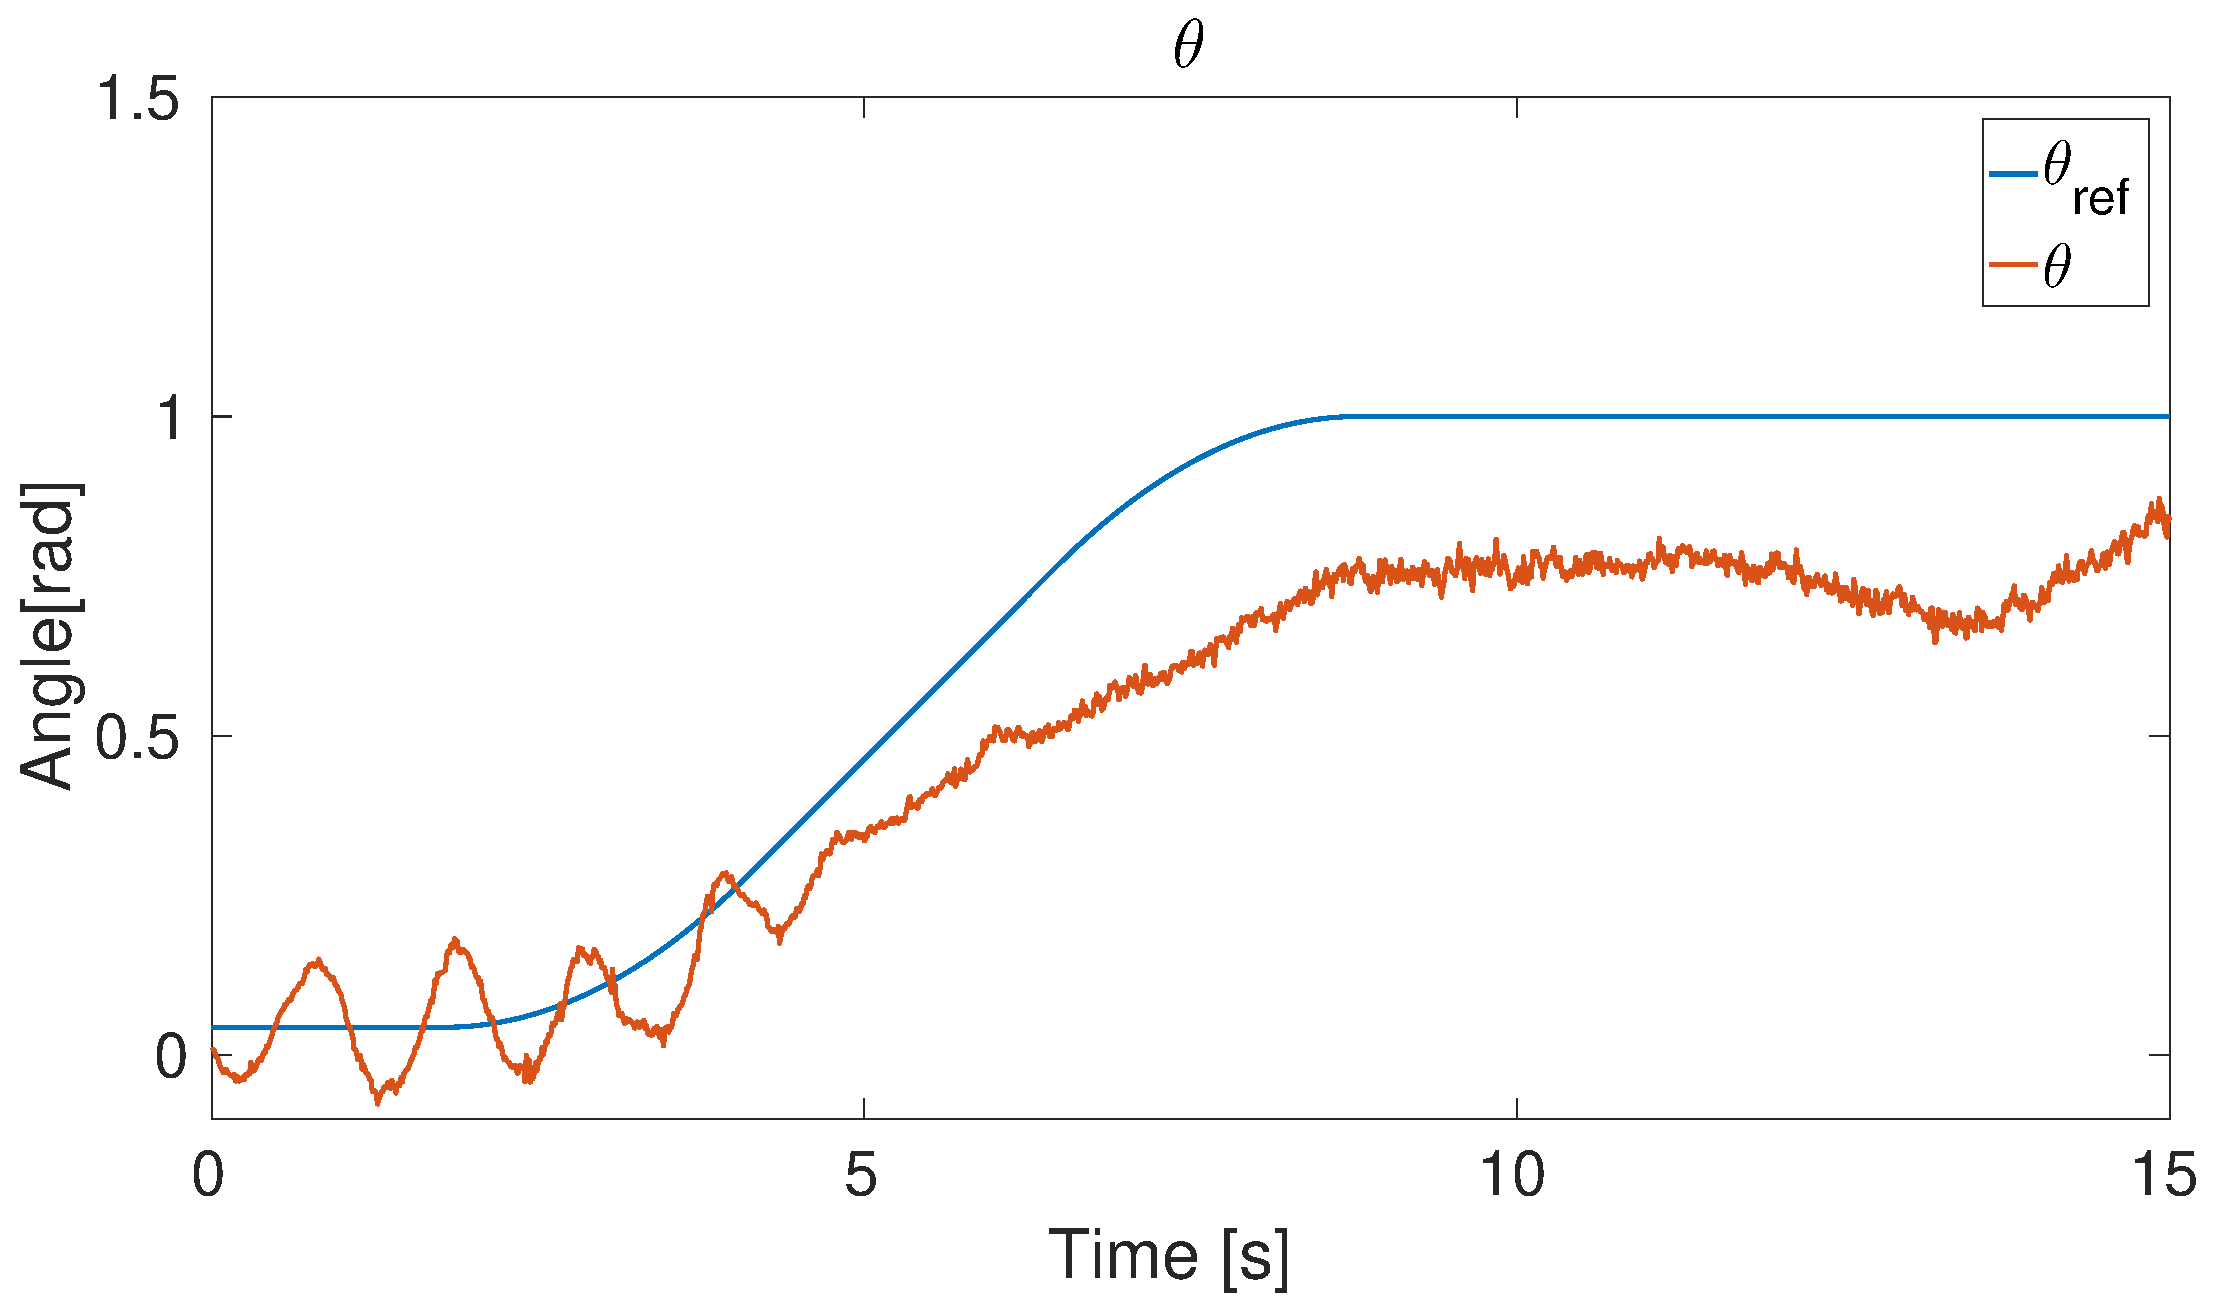
\includegraphics[scale=0.28]{../Master/fig/testStepThetaPhiThetas3e10a1}
}
\end{frame}




%%%%%%%%%Conclusion%%%%%%%%%%%%%%%%%%%%%%%%%%%%%%%%%%%%%%%%%%%%%%%%%%%%%%%%%%%%%%%%%%
\section{Conclusion}
\begin{frame}

\end{frame}
%%%%%%%%%%%%

\end{document}
